\documentclass[english,a4paper]{csuserguide}
\usepackage{epsfig}
\usepackage{epstopdf}
\usepackage{url}
\usepackage[latin1]{inputenc}
\usepackage{babel}
\usepackage{listings}
\usepackage{color}
\usepackage{moreverb}
\usepackage{colortbl}
\usepackage{textcomp}
\usepackage{xspace} 
\usepackage[colorlinks=true]{hyperref}

\definecolor{gray}{gray}{0.5}
\definecolor{key}{rgb}{0,0.5,0} 
\definecolor{darkgreen}{cmyk}{0.7, 0, 1, 0.5}
\definecolor{darkblue}{cmyk}{1, 0.8, 0, 0}
\definecolor{lightblue}{cmyk}{0.05,0,0,0.05}
\definecolor{grey}{cmyk}{0.1,0.1,0.1,1}
\definecolor{lightgrey}{cmyk}{0,0,0,0.5}
\definecolor{purple}{cmyk}{0.8,1,0,0}

\providecommand{\version}{DEV}% fallback definition
\providecommand{\vertag}{CS-USERGUIDE-DEV-DRAFT}% fallback definition

% begin definition of common keywords
\newcommand{\MsgTree}{\textit{MsgTree}\xspace}
\newcommand{\NodeSet}{\textit{NodeSet}\xspace}
\newcommand{\RangeSet}{\textit{RangeSet}\xspace}
\newcommand{\Task}{\textit{Task}\xspace}
\newcommand{\Engine}{\textit{Engine}\xspace}
\newcommand{\nodeset}{\texttt{nodeset}\xspace}
\newcommand{\clush}{\texttt{clush}\xspace}
\newcommand{\clubak}{\texttt{clubak}\xspace}
% end of common keywords

\newcommand{\nautphoto}{
\begin{center}
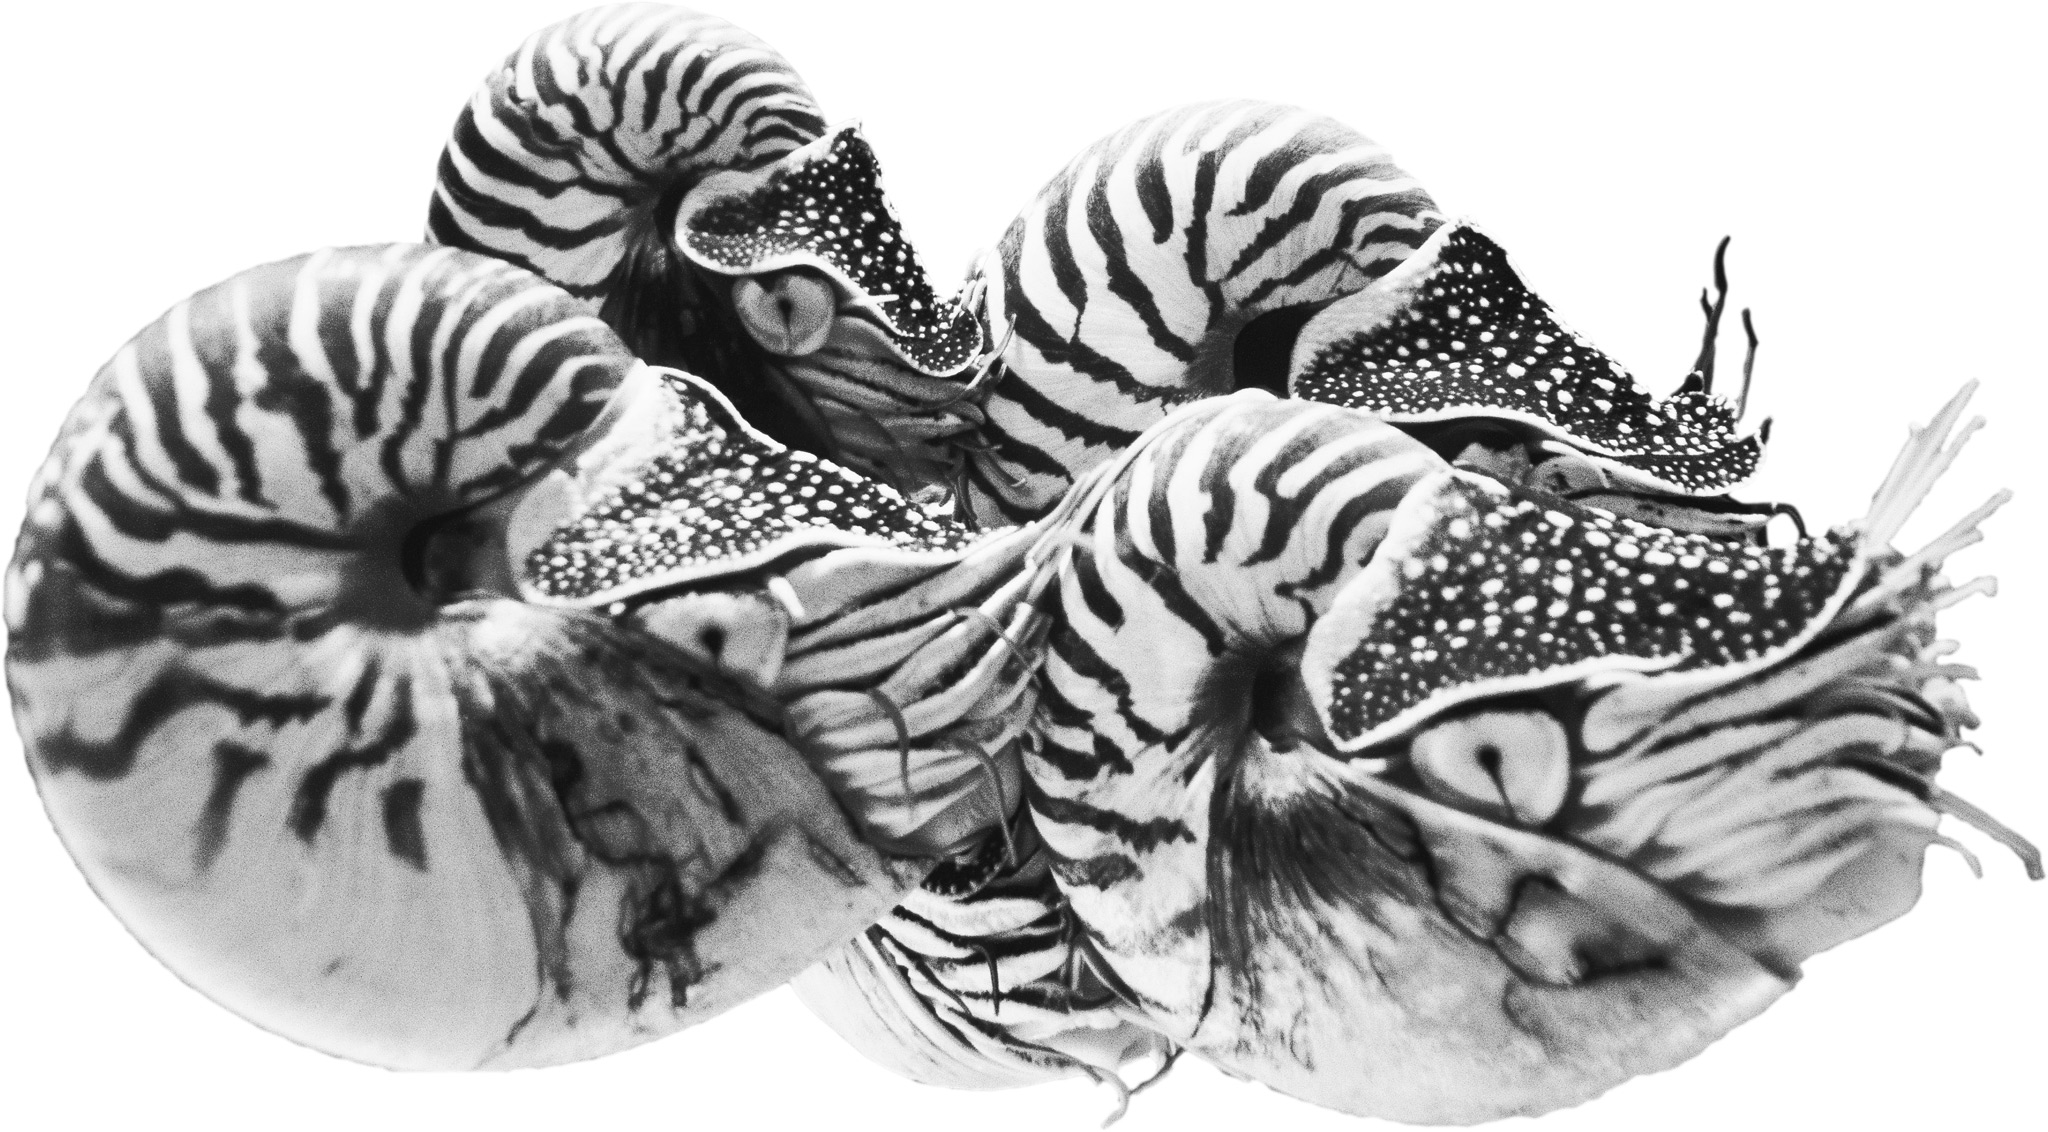
\includegraphics[scale=0.2]{clustershell-naut-bw}

\scriptsize{\textsf{Photo: Todd Anderson}}
\end{center}
}

\newcommand{\declareheaders}{
  \lhead{
    \emph{ClusterShell User and Programming Guide (v\version)}
  }
  \rhead{
    \normalsize {\thepage}/\pageref{LastPage}
  }
}

\pdfinfo
{ /Title (ClusterShell User and Programming Guide (v\version))
  /Creator (LaTeX)
  /Producer (pdfLaTeX)
  /Author (S. THIELL)
  /CreationDate (D:20110912)
  /ModDate (D: 20120408)
  /Keywords (ClusterShell, clush, shell, nodeset, Python, HPC, Linux)
}

\title{ClusterShell v\version}

\author{St\'ephane \textsc{Thiell}\\
Aur\'elien \textsc{Degr\'emont}
}

\newcommand{\lstsetconfig}{
\lstset{
language=python,
basicstyle=\ttfamily\small,
%otherkeywords={1, 2, 3, 4, 5, 6, 7, 8 ,9 , 0, -, =, +, [, ], \{, \}, :, *, !},
keywordstyle=\bfseries\color{darkblue},
stringstyle=\color{purple},
showstringspaces=false,
emph={genders, class, pass, in, for, while, if, is, elif, else, not, and, or,
def, print, exec, break, continue, return},
emphstyle=\color{red}\bfseries,
emph={[2] \$GROUP, \$NODE},
emphstyle=[2]\color{key},
emph={[3] default, groupsdir, map, all, list, reverse},
emphstyle=[3]\color{blue},
upquote=true,
tabsize=4,
morecomment=[s]{"""}{"""},
commentstyle=\color{darkgreen}\slshape,
framexleftmargin=1mm, framextopmargin=1mm, frame=shadowbox,
rulesepcolor=\color{lightgrey},
numberstyle=\footnotesize\color{grey}
}
}

\newcommand{\lstsetpython}{
\lstset{
language=python,
basicstyle=\ttfamily\small,
%otherkeywords={1, 2, 3, 4, 5, 6, 7, 8 ,9 , 0, -, =, +, [, ], \{, \}, :, *, !},
keywordstyle=\bfseries\color{darkblue},
stringstyle=\color{purple},
showstringspaces=false,
emph={class, pass, in, for, while, if, is, elif, else, not, and, or,
def, print, exec, break, continue, return},
emphstyle=\color{red}\bfseries,
emph={[2]True, False, None, self},
emphstyle=[2]\color{key},
emph={[3]from, import, as},
emphstyle=[3]\color{blue},
upquote=true,
tabsize=4,
morecomment=[s]{"""}{"""},
commentstyle=\color{darkgreen}\slshape,
framexleftmargin=1mm, framextopmargin=1mm, frame=shadowbox,
rulesepcolor=\color{lightgrey},
numberstyle=\footnotesize\color{grey}
}
}

\newcommand{\lstsetbash}{
\lstset{
language=bash,
basicstyle=\ttfamily\small,
otherkeywords={xargs, ssh, ls, sinfo, sacct, mount, cut},
keywordstyle=\bfseries\color{darkblue},
stringstyle=\color{purple},
showstringspaces=false,
emph={class, pass, in, for, while, if, is, elif, else, not, and, or,
def, print, exec, break, continue, return, do, done},
emphstyle=\color{red}\bfseries,
emph={[2]true, false, None, self, expand, fold, regroup, list, count},
emphstyle=[2]\color{key},
emph={[3]from, import, as, clush, nodeset, clubak},
emphstyle=[3]\color{blue},
upquote=true,
tabsize=4,
morecomment=[s]{"""}{"""},
commentstyle=\color{darkgreen}\slshape,
framexleftmargin=1mm, framextopmargin=1mm, frame=shadowbox,
rulesepcolor=\color{lightgrey},
numberstyle=\footnotesize\color{grey}
}
}

\setlength\parindent{0pt}

\begin{document}
\parskip 7.2pt

\maketitle

\fancyfoot[C]{\thepage}

\tableofcontents

\parskip 10.8pt

\section*{Introduction}
\addcontentsline{toc}{section}{Introduction}

\indent ClusterShell provides a light, unified and robust command execution Python framework, well-suited to ease daily administrative tasks of nowadays Linux clusters. Some of the most important benefits of using ClusterShell are:
\begin{itemize}
\item{to provide an efficient, parallel and highly scalable command execution engine in Python,}
\item{to provide an unified node groups syntax and external group access (see the NodeSet class),}
\item{to significantly speed up initial cluster setup and daily administrative tasks when using tools like \textbf{clush} and \textbf{nodeset}.}
\end{itemize}

Created by the HPC Linux system development team at CEA\footnote{French Alternative Energies and Atomic Energy Commission, a leading technological research organization in Europe (\url{http://www-hpc.cea.fr/index-en.htm})} HPC center in France, ClusterShell is designed around medium and long term ideas of sharing cluster administration development time, and this according to two axes:
\begin{itemize}
\item{sharing administrative applications between main components of the computing center: compute clusters, but also storage clusters and server farms (so they can use the same efficient framework for their administrative applications),}
\item{sharing administration techniques across multiple generations of super-computing clusters (first of all, to avoid that every cluster administration application has to implement its own command execution layer, but also to encourage the adoption of event-based coding model in administration scripts).}
\end{itemize}

Two available coding models make the library well-suited for simple scripts or for complex applications as well. Also, the library is fully cluster-aware and has primarily been made for executing remote shell commands in parallel and gathering output results. But it now also provides the developer a set of extra features for administrative applications, like file copy support or time-based notifications (timers) which are discussed in this document.

\newpage
\part{Installation}

In this part, we address ClusterShell installation information first. Then, ClusterShell user tools are documented. Indeed, three Python scripts using the ClusterShell library are provided with the distribution:
\begin{itemize}
\item \nodeset: a tool to manage cluster node sets and groups,
\item \clush: a powerful parallel command execution tool with output gathering,
\item \clubak: a tool to gather and display results from clush/pdsh-like output (and more).
\end{itemize}


\section{Requirements}

ClusterShell v\version{} should work with any Unix\footnote{Unix in the same sense of the \textit{"Availability: Unix"} notes in the Python documentation} operating systems which provides Python 2.4 to 2.7 (not Python 3.0 validated) and OpenSSH or any compatible Secure Shell clients.

Furthermore, ClusterShell's engine has been optimized when the \verb+poll()+ syscall is available or even better, when the \verb+epoll_wait()+ syscall (like in Linux 2.6) is available.

For instance, ClusterShell v\version{} is known to work on the following operating systems:
\begin{itemize}
\item GNU/Linux RedHat EL5 or CentOS 5.x (Python 2.4) and EL6 (Python 2.6)
\item GNU/Linux Fedora 11, 12, 13 (Python 2.6), 14, 15 and 16 (Python 2.7)
\item GNU/Linux Debian (wheezy and sid)
\item Mac OS X 10.5.8 (Python 2.5.1)
\end{itemize}

\section{Distribution}
\lstsetbash

ClusterShell is an open-source project distributed under the CeCILL-C flavor of the CeCILL license family\footnote{\url{http://www.cecill.info/index.en.html}}, which is in conformance with the French law and compatible with the GNU LGPL (Lesser GPL) license, which means that many possibilities are offered to the end user. Also, as a software library, ClusterShell has to remain easily available to everyone. Hopefully, packages are currently maintained in Fedora Linux, RHEL (through EPEL repositories) and Debian.

\subsection{Fedora}

At the time of writing, ClusterShell v\version{} is available on Fedora 15 and 16 (releases being maintained by the Fedora Project).

\paragraph{Install ClusterShell from \textit{Fedora Updates}}

ClusterShell is part of Fedora, so it is really easy to install it with \textit{yum}, although you have to keep the Fedora \textit{updates} default repository. The following command checks whether the packages are available on a Fedora machine:

\begin{verbatim}
# yum list \*clustershell
Loaded plugins: presto, priorities, refresh-packagekit
Available Packages
clustershell.noarch                        1.5.1-1.fc15                  updates
vim-clustershell.noarch                    1.5.1-1.fc15                  updates
\end{verbatim}

Then, install ClusterShell (library and tools) with the following command:
\begin{verbatim}
# yum install clustershell vim-clustershell
\end{verbatim}

Please note that optional (but recommended) \verb+vim-clustershell+ package will install VIM syntax files for ClusterShell configuration files like \verb+clush.conf+ and \verb+groups.conf+.

\paragraph{Install ClusterShell from \textit{Fedora Updates Testing}}

Recent releases of ClusterShell are first available through the Test Updates\footnote{\url{http://fedoraproject.org/wiki/QA/Updates_Testing}} \textit{yum} repository of Fedora, then it is later\footnote{testing time is about one week later for Fedora, two weeks for EPEL packages} pushed to the stable \textit{updates} repository. The following \textit{yum} command will also checks for packages availability in the \textit{updates-testing} repository:

\begin{verbatim}
# yum list \*clustershell --enablerepo=updates-testing
\end{verbatim}

To install, also add the \verb+--enablerepo=updates-testing+ option, for instance:
\begin{verbatim}
# yum install clustershell vim-clustershell --enablerepo=updates-testing
\end{verbatim}

\subsection{Red Hat Enterprise Linux (and CentOS)}

ClusterShell packages are maintained on Extra Packages for Enterprise Linux (EPEL\footnote{\url{http://fedoraproject.org/wiki/EPEL}}) for Red Hat Enterprise Linux (RHEL) and its compatible spinoffs such as CentOS or Scientific Linux. At the time of writing, ClusterShell v\version{} is available on EPEL 5 and EPEL 6.


\paragraph{Install ClusterShell from EPEL}

First you have to enable the \textit{yum} EPEL repository. We advice you to download and install the EPEL repository RPM package\footnote{\url{http://download.fedora.redhat.com/pub/epel/6/x86_64/repoview/epel-release.html}}.

Then, the ClusterShell installation procedure is quite the same of the Fedora \textit{Updates} one, for instance:

\begin{verbatim}
# yum install clustershell vim-clustershell
\end{verbatim}

\subsection{Debian}

ClusterShell is available in Debian since the "wheezy" testing release (February 2011):
\begin{itemize}
\item{\url{http://packages.debian.org/wheezy/clustershell}}
\item{\url{http://packages.debian.org/sid/clustershell}}
\end{itemize}

To install it on Debian, simply use:

\verb+# apt-get install clustershell+


\subsection{Ubuntu}

Like Debian, it is easy to get and install ClusterShell on Ubuntu (also with \verb+apt-get+). To do so, please first enable the \textbf{universe} repository. ClusterShell is available since "Natty" release (11.04):
\begin{itemize}
\item{\url{http://packages.ubuntu.com/clustershell}}
\end{itemize}

\subsection{General distribution (Sourceforge \& Github)}

ClusterShell is distributed in several packages. On RedHat-like OS, we recommend to use the RPM  package (.rpm) distribution. General distribution source packages and RPM package are available on the Sourceforge.net download page:

\url{http://sourceforge.net/projects/clustershell/files/clustershell/}

There is no difference between Fedora (or EPEL) RPM packages and the ones found on Sourceforge.

\medskip

Current source is also available through Git, use the following command to retrieve the latest development version from the repository:
\begin{verbatim}
$ git clone git@github.com:cea-hpc/clustershell.git
\end{verbatim}

Install ClusterShell as a standard Python package (may need to be root):

\begin{verbatim}
# tar -xzf clustershell-\version{}.tar.gz
# cd clustershell-\version{}
# python setup.py install
\end{verbatim}

Then, you should create \verb+/etc/clustershell+ and put in it files found in conf directory. This is the same thing when using pip\footnote{pip is a tool for installing and managing Python packages, such as those found in the Python Package Index}. This should be fixed in a future release.

\newpage

\lstsetbash

\part{Tools}

\section{nodeset}
\label{nodeset-tool}

The \nodeset command enables easy manipulation of node sets, as well as node groups, at the command line level. As it is very user-friendly and efficient, the \nodeset command can quickly improve traditional cluster shell scripts. It is also full-featured as it provides most of the \NodeSet  and \RangeSet class methods (see section \ref{class-NodeSet} page \pageref{class-NodeSet} for \NodeSet, and \ref{class-RangeSet} page \pageref{class-RangeSet} for \RangeSet).

This section will guide you through the basics and also advanced features of \nodeset.

\subsection{Usage basics}
\label{nodeset-commands}

One exclusive command must be specified to \nodeset, for example:

\bigskip

\begin{lstlisting}[breaklines=true, breakatwhitespace=true] 
$ nodeset --expand node[13-15,17-19]
node13 node14 node15 node17 node18 node19
$ nodeset --count node[13-15,17-19]
6
$ nodeset --fold node1-ipmi node2-ipmi node3-ipmi
node[1-3]-ipmi
\end{lstlisting}


\subsubsection{Commands with inputs}

Some  \nodeset commands require input (eg. node names, node sets or node groups), and some only give output. The following table shows commands that require some input:

\begin{center}
\label{nodeset-cmds}
\begin{tabular}{|p{3.2cm}|p{13.2cm}|} 
\hline 
\textbf{Command} & \textbf{Description} \\
\hline
\verb+-c, --count+& Count and display the total number of nodes in node sets or/and node groups.\\
\hline
\verb+-e, --expand+ & Expand node sets or/and node groups as unitary node names separated by the interpreted string specified with \verb+-S+ (default is the space character\mbox{ " "}), for example:
\lstinline+$ nodeset -e -S'\n' node[0-3]+\\
\hline
\verb+-f, --fold+ & Fold (compact) node sets or/and node groups into one set of nodes (by previously resolving any groups). The resulting node set is guaranteed to be free from node group (see \verb+--regroup+ below if you want to resolve node groups in result).\\
\hline
\verb+-r, --regroup+ & Fold (compact) node sets or/and node groups into one set of nodes using node groups whenever possible (by previously resolving any groups). See \textit{Working with node groups}, section~\ref{nodeset-groups} page~\pageref{nodeset-groups}.\\
\hline
\end{tabular}
\end{center}


There are three ways to give some input to the \nodeset command:
\begin{itemize}
\item{from command line arguments,}
\item{from standard input (enabled when no arguments are found on command line),}
\item{from both command line and standard input, by using the special argument \verb+"-"+.}
\end{itemize}

The following example illustrates the three ways to feed \nodeset:
\bigskip

\begin{lstlisting}[breaklines=true, breakatwhitespace=true] 
$ nodeset -f node1 node6 node7
node[1,6-7]

$ echo node1 node6 node7 | nodeset -f
node[1,6-7]

$ echo node1 node6 node7 | nodeset -f node0 -
node[0-1,6-7]
\end{lstlisting}

\label{nodeset-stdin}
Furthermore, \nodeset's standard input reader is able to process multiple lines and multiple node sets or groups per line. The following example shows a simple use case:
\bigskip

\begin{lstlisting}[breaklines=true, breakatwhitespace=true] 
$ mount -t nfs | cut -d':' -f1
nfsserv1
nfsserv2
nfsserv3

$ mount -t nfs | cut -d':' -f1 | nodeset -f
nfsserv[1-3]
\end{lstlisting}


Other usage examples of \nodeset below show how it can be useful to provide node sets from standard input (\verb+sinfo+ is a SLURM\footnote{SLURM is an open-source resource manager (\url{https://computing.llnl.gov/linux/slurm/})} command to view nodes and partitions information and \verb+sacct+ is a command to display SLURM accounting data):
\bigskip

\begin{lstlisting}[breaklines=true, breakatwhitespace=true] 
$ sinfo -p cuda -o '%N' -h
node[156-159]

$ sinfo -p cuda -o '%N' -h | nodeset -e
node156 node157 node158 node159

$ for node in $(sinfo -p cuda -o '%N' -h | nodeset -e); do
	sacct -a -N $node > /tmp/cudajobs.$node;
  done

\end{lstlisting}

Previous rules also apply when working with node groups, for example when using \verb+nodeset -r+ reading from standard input (and a matching group is found):
\medskip
\begin{lstlisting}[breaklines=true, breakatwhitespace=true] 
$ nodeset -f @gpu
node[156-159]

$ sinfo -p cuda -o '%N' -h | nodeset -r
@gpu
\end{lstlisting}


\subsubsection{Commands with no input}

The following table shows all other commands that are supported by \nodeset. These commands don't support any input (like node sets), but can still recognize options as specified below.
\label{nodeset-grpcmd}

\begin{center}
\label{nodeset-cmds2}
\begin{tabular}{|p{3.2cm}|p{13.2cm}|} 
\hline 
\textbf{Command with no input} & \textbf{Description} \\
\hline
\verb+-l, --list+ & List node groups from selected \textit{group source} as specified with \verb+-s+ or \verb+--groupsource+. If not specified, node groups from the default \textit{group source} are listed (see section \ref{groups-config} page~\pageref{groups-config} for default \textit{group source} configuration).\\
\hline
\verb+--groupsources+ & List all configured \textit{group sources}, one per line, as configured in \textit{groups.conf} (see section \ref{groups-config} page~\pageref{groups-config}). The default \textit{group source} is appended with \mbox{" (default)"}, unless the \verb+-q+ (\verb+--quiet+) option is specified. This command is  mainly here to avoid reading any configuration files, or to check if all work fine when configuring \textit{group sources}.\\
\hline
\end{tabular}
\end{center}

\subsection{Stepping and auto-stepping}
\label{nodeset-stepping}

The \nodeset command, as does the \clush command, is able to recognize by default a factorized notation for range sets of the form \verb+a-b/c+, indicating a list of integers starting from \verb+a+, less than or equal to \verb+b+ with the increment (step) \verb+c+.

For example, the \verb+0-6/2+ format indicates a range of 0-6 stepped by 2; that is 0,2,4,6.
\medskip
\begin{lstlisting}[breaklines=true, breakatwhitespace=true] 
$ nodeset -e node[0-6/2]
node0 node2 node4 node6
\end{lstlisting}

However, by default, \nodeset never uses this stepping notation in output results, as other cluster tools seldom if ever support this feature. Thus, to enable such factorized output in \nodeset, you must specify \verb+--autostep=AUTOSTEP+ to set an auto step threshold number when folding nodesets (ie. when using \verb+-f+ or \verb+-r+). This threshold number (\verb+AUTOSTEP+) is the minimum occurrence of equally-spaced integers needed to enable auto-stepping.

\newpage
For example:
\medskip
\begin{lstlisting}[breaklines=true, breakatwhitespace=true] 
$ nodeset -f --autostep=3 node1 node3 node5
node[1-5/2]

$ nodeset -f --autostep=4 node1 node3 node5
node[1,3,5]
\end{lstlisting}

It is important to note that resulting node sets with enabled auto-stepping never create overlapping ranges, for example:
\medskip
\begin{lstlisting}[breaklines=true, breakatwhitespace=true] 
$ nodeset -f --autostep=3 node1 node5 node9 node13
node[1-13/4]
$ nodeset -f --autostep=3 node1 node5 node7 node9 node13
node[1,5-9/2,13]
\end{lstlisting}

However, any ranges given as input may still overlap (in this case, \nodeset will automatically spread them out so that they do not overlap), for example:
\medskip
\begin{lstlisting}[breaklines=true, breakatwhitespace=true] 
$ nodeset -f --autostep=3 node[1-13/4,7]                
node[1,5-9/2,13]
\end{lstlisting}

\subsection{Zero-padding}
\label{nodeset-zpad}

Sometimes, cluster node names are padded with zeros (eg. \textit{"node007"}). With \nodeset, when leading zeros are used, resulting host names or node sets are automatically padded with zeros as well. For example:
\medskip
\begin{lstlisting}[breaklines=true, breakatwhitespace=true]
$ nodeset -e node[08-11]
node08 node09 node10 node11

$ nodeset -f node001 node002 node003 node005
node[001-003,005]
\end{lstlisting}

Zero-padding and stepping (as seen in section \ref{nodeset-stepping}) together are also supported, for example:
\medskip
\begin{lstlisting}[breaklines=true, breakatwhitespace=true]
$ nodeset -e node[000-012/4]
node000 node004 node008 node012
\end{lstlisting}

Nevertheless, care should be taken when dealing with padding, as a zero-padded node name has priority over a normal one, for example:
\medskip
\begin{lstlisting}[breaklines=true, breakatwhitespace=true]
$ nodeset -f node1 node02
node[01-02]
\end{lstlisting}

To clarify, \nodeset will always try to coalesce node names by their numerical index first (without taking care of any zero-padding), and then will use the first zero-padding rule encountered. In the following example, the first zero-padding rule found is \verb+node01+'s one:
\medskip
\begin{lstlisting}[breaklines=true, breakatwhitespace=true]
$ nodeset -f node01 node002
node[01-02]
\end{lstlisting}

That said, you can see it is not possible to mix \verb+node01+ and \verb+node001+ in the same node set (not supported by the \NodeSet class), but that would be a tricky case anyway.


\subsection{Arithmetic operations}
\label{nodeset-arithmetic}

As a preamble to this section, keep in mind that all operations can be repeated/mixed within the same \nodeset command line, they will be processed from left to right.

\subsubsection{Union operation}
Union is the easiest arithmetic operation supported by \nodeset: there is no special command line option for that, just provide several node sets and the union operation will be computed, for example:
\medskip
\begin{lstlisting}[breaklines=true, breakatwhitespace=true]
$ nodeset -f node[1-3] node[4-7]
node[1-7]

$ nodeset -f node[1-3] node[2-7] node[5-8]  
node[1-8]
\end{lstlisting}


\subsubsection{Other operations}
As an extension to the above, other arithmetic operations are available by using the following command-line options (\textit{working set} is the node set currently processed on the command line -- always from left to right):
\begin{center}
\label{nodeset-ops}
\begin{tabular}{|p{5.4cm}|p{11cm}|} 
\hline 
\textbf{Command option} & \textbf{Operation} \\
\hline
\verb+-x +\textit{NODESET} \verb+--exclude=+\textit{NODESET}& \textbf{exclusion}: compute a new set with elements in \textit{working set} but not in \textit{NODESET}\\
\hline
\verb+-i +\textit{NODESET} \verb+--intersection=+\textit{NODESET}& \textbf{intersection}: compute a new set with elements common to \textit{working set} and \textit{NODESET}\\
\hline
\verb+-X +\textit{NODESET} \verb+--xor=+\textit{NODESET}& \textbf{symmetric difference}: compute a new set with elements that are in exactly one of the \textit{working set} and \textit{NODESET}\\
\hline
\end{tabular}
\end{center}

If rangeset mode (\verb+-R+) is turned on, all arithmetic operations are supported by replacing \textit{NODESET} by any \textit{RANGESET}. See section \ref{nodeset-rangeset} (page~\pageref{nodeset-rangeset}) for more info about \nodeset's rangeset mode.


Arithmetic operations usage examples:
\medskip
\begin{lstlisting}[breaklines=true, breakatwhitespace=true]
$ nodeset -f node[1-9] -x node6
node[1-5,7-9]

$ nodeset -f node[1-9] -i node[6-11]
node[6-9]

$ nodeset -f node[1-9] -X node[6-11]
node[1-5,10-11]

$ nodeset -f node[1-9] -x node6 -i node[6-12]
node[7-9]
\end{lstlisting}


\subsubsection{\textit{Extended patterns} support}
\label{nodeset-extended-patterns}
\nodeset does also support arithmetic operations through its "extended patterns" (inherited from NodeSet extended pattern feature, see section \ref{class-NodeSet-extended-patterns} page \pageref{class-NodeSet-extended-patterns}),  there is an example of use:
\medskip
\begin{lstlisting}[breaklines=true, breakatwhitespace=true]
$ nodeset -f node[1-4],node[5-9]
node[1-9]

$ nodeset -f node[1-9]\!node6   
node[1-5,7-9]
\end{lstlisting}

\begin{lstlisting}[breaklines=true, breakatwhitespace=true]
$ nodeset -f node[1-9]\&node[6-12]
node[6-9]

$ nodeset -f node[1-9]^node[6-11]
node[1-5,10-11]
\end{lstlisting}

\subsection{Special operations}
\label{nodeset-special}

Three special operations are currently available: node set slicing, splitting on a predefined node count and splitting non-contiguous subsets. There are all explained below.

\subsubsection{Slicing}
\label{nodeset-slice}

Slicing is a way to select elements from a node set (or a range set when using \verb+-R+ toggle option, see section \ref{nodeset-rangeset}, page~\pageref{nodeset-rangeset}) by their index. In this case actually, and because \nodeset's underlying \textit{NodeSet} class sorts elements as observed after folding (for example), the word \textit{set} may sound like a stretch of language (a \textit{set} isn't usually sorted). Indeed, \textit{NodeSet} further guarantees that its iterator will traverse the set in order, so we should see it as a \textit{sorted set} (see page \pageref{class-NodeSet}).  The following simple example illustrates this sorting behavior:

\medskip
\begin{lstlisting}[breaklines=true, breakatwhitespace=true]
$ nodeset -f b2 b1 b0 b c a0 a
a,a0,b,b[0-2],c
\end{lstlisting}

Slicing is performed through the following command-line option:
\begin{center}
\begin{tabular}{|p{5.4cm}|p{11.4cm}|} 
\hline 
\textbf{Option} & \textbf{Operation} \\
\hline
\verb+-I +\textit{RANGESET} \verb+--slice=+\textit{RANGESET}& \textbf{slicing}: get sliced off result, selecting elements from provided rangeset's indexes\\
\hline
\end{tabular}
\end{center}

Some slicing examples are shown below:
\medskip
\begin{lstlisting}[breaklines=true, breakatwhitespace=true]
$ nodeset -f -I 0 node[4-8]
node4

$ nodeset -f --slice=0 bnode[0-9] anode[0-9]
anode0

$ nodeset -f --slice=1,4,7,9,15 bnode[0-9] anode[0-9]
anode[1,4,7,9],bnode5

$ nodeset -f --slice=0-18/2 bnode[0-9] anode[0-9]
anode[0,2,4,6,8],bnode[0,2,4,6,8]
\end{lstlisting}


\subsubsection{Splitting into \textit{n} subsets}
\label{nodeset-splitting-n}
Splitting a node set into several parts is often useful to get separate groups of nodes, for instance when you want to check MPI comm between nodes, etc. Based on \NodeSet's \lstinline+split()+ method (see section~\ref{class-NodeSet-split} page~\pageref{class-NodeSet-split}), the \nodeset command provides the following additional command-line option (since v1.4):
\begin{center}
\label{nodeset-split}
\begin{tabular}{|p{5.4cm}|p{11.4cm}|} 
\hline 
\textbf{Option} & \textbf{Operation} \\
\hline
\verb+--split=+\textit{MAXSPLIT}& \textbf{splitting}: split result into a number of subsets\\
\hline
\end{tabular}
\end{center}

\textit{MAXSPLIT} is an integer specifying the number of separate groups of nodes to compute. Input's node set is divided into smaller groups, whenever possible with the same size (only the last ones may be smaller due to rounding). Obviously, if \mbox{\textit{MAXSPLIT}} is higher than or equal to the number N of elements in the set, then the set is split to N single sets.

\newpage
Some node set splitting examples:
\medskip
\begin{lstlisting}[breaklines=true, breakatwhitespace=true]
$ nodeset -f --split=4 node[0-7]
node[0-1]
node[2-3]
node[4-5]
node[6-7]

$ nodeset -f --split=4 node[0-6]
node[0-1]
node[2-3]
node[4-5]
node6

$ nodeset -f --split=10000 node[0-4]
foo0
foo1
foo2
foo3
foo4

$ nodeset -f --autostep=3 --split=2 node[0-38/2]
node[0-18/2]
node[20-38/2]
\end{lstlisting}


\subsubsection{Splitting off non-contiguous subsets}
\label{nodeset-splitting-contiguous}
It can be useful to split a node set into several contiguous subsets (with same pattern name and contiguous range indexes, eg. "\verb+node[1-100]+"). Since v1.6, the \verb+--contiguous+ option allows you to do that. It is based on \NodeSet's \lstinline+groups()+ method (see section~\ref{class-NodeSet-contiguous} page~\pageref{class-NodeSet-contiguous}), and should be specified with standard commands (fold, expand, count, regroup). The following example shows how to split   off non-contiguous subsets of a specified node set, and to display each resulting contiguous node set in a folded manner to separated lines:
\bigskip

\begin{lstlisting}[breaklines=true, breakatwhitespace=true]
$ nodeset -f --contiguous node[1-100,200-300,500]
node[1-100]
node[200-300]
node500
\end{lstlisting}

Similarly, the following example shows how to display each resulting contiguous node set in an expanded manner to separate lines:
\bigskip

\begin{lstlisting}[breaklines=true, breakatwhitespace=true]
$ nodeset -e --contiguous node[1-9,11-19]
node1 node2 node3 node4 node5 node6 node7 node8 node9
node11 node12 node13 node14 node15 node16 node17 node18 node19
\end{lstlisting}


\subsection{Node groups}
\label{nodeset-groups}

This section tackles the node groups feature available more particularly through the \nodeset command-line tool. The ClusterShell library defines a node groups syntax and allow you to bind these group sources to your applications (cf. \ref{groups-config} page~\pageref{groups-config}). Having those group sources, group provisioning is easily done through user-defined external shell commands. Thus, node groups might be very dynamic and their nodes might change very often\footnote{However, for performance reasons, external call results are still cached in memory to avoid duplicate external calls during \lstinline+nodeset+ execution.}. For example, a group source can be bound to a resource manager or a custom cluster database.

For further details about using node groups in Python, please see section~\ref{class-NodeSet-groups} page~\pageref{class-NodeSet-groups}. For advanced usage, you should also be able to define your own group source directly in Python (cf. section~\ref{class-NodeSet-groups-override} page~\pageref{class-NodeSet-groups-override}).

\subsubsection{Node group expression rules}
\label{nodeset-groupsexpr}

The general node group expression is \verb+@source:groupname+. For example, \verb+@slurm:bigmem+ represents the group \textit{"bigmem"} of the group source \textit{"slurm"}. Moreover, a shortened expression is available when using the default group source (defined by configuration); for instance \verb+@compute+ represents the \textit{"compute"} group of the default group source.

Valid group source names and group names can contain alphanumeric characters, hyphens and underscores (no space allowed). Indeed, same rules apply to node names.

\subsubsection{Listing group sources}
As already mentioned in section \ref{nodeset-grpcmd} page \pageref{nodeset-grpcmd}, the following \nodeset command is available to list configured group sources and also display the default group source (unless \verb+-q+ is provided):
\medskip
\begin{lstlisting}[breaklines=true, breakatwhitespace=true]
$ nodeset --groupsources
local(default)
genders
slurm
\end{lstlisting}

\pagebreak[2]

\subsubsection{Listing group names}
\label{nodeset-group-list}
If the \textbf{list} external shell command is configured (see section \ref{groups-config} page~\pageref{groups-config}), it is possible to list available groups (from the default source) with the following commands:
\medskip
\begin{lstlisting}[breaklines=true, breakatwhitespace=true]
$ nodeset -l
@mgnt
@mds
@oss
@login
@compute
\end{lstlisting}

Or, to list groups from a specific group source, use:
\medskip
\begin{lstlisting}[breaklines=true, breakatwhitespace=true]
$ nodeset -l -s slurm
@slurm:parallel
@slurm:cuda
\end{lstlisting}

You can also use \lstinline+nodeset -ll+ to see each group's associated node sets.

\subsubsection{Using node groups in basic commands}

The use of node groups with the \nodeset command is very straightforward. Indeed, any group name, prefixed by "\verb+@+" as mentioned above, can be used in lieu of a node name, where it will be substituted for all nodes in that group.

A first, simple example is a group expansion (using default source) with \nodeset:
\medskip
\begin{lstlisting}[breaklines=true, breakatwhitespace=true]
$ nodeset -e @oss
node40 node41 node42 node43 node44 node45
\end{lstlisting}

The \nodeset count command works as expected:
\medskip
\begin{lstlisting}[breaklines=true, breakatwhitespace=true]
$ nodeset -c @oss
6
\end{lstlisting}

Also \nodeset's folding command can always resolve node groups:
\medskip
\begin{lstlisting}[breaklines=true, breakatwhitespace=true]
$ nodeset -f @oss
node[40-45]
\end{lstlisting}

There are usually two ways to use a specific group source (need to be properly configured):
\medskip
\begin{lstlisting}[breaklines=true, breakatwhitespace=true]
$ nodeset -f @slurm:parallel
node[50-81]

$ nodeset -f -s slurm @parallel
node[50-81]
\end{lstlisting}

\pagebreak[4]

\subsubsection{Finding node groups}
\label{nodeset-group-finding}
As an extension to the \textbf{list} command (as seen in section~\ref{nodeset-group-list} page~\pageref{nodeset-group-list}), you can search node groups that a specified node set belongs to with \lstinline+nodeset -l[ll]+ as follow:
\medskip
\begin{lstlisting}[breaklines=true, breakatwhitespace=true]
$ nodeset -l node40
@all
@oss

$ nodeset -ll node40
@all node[1-159]
@oss node[40-45]
\end{lstlisting}

\lstsetpython
This feature is implemented with the help of the \lstinline+NodeSet.groups()+ method (see section~\ref{class-NodeSet-groups-finding} page~\pageref{class-NodeSet-groups-finding} for further details).

\subsubsection{Resolving node groups}
\label{nodeset-regroup}
\lstsetpython
If needed group configuration conditions are met (cf. \ref{groups-config} page~\pageref{groups-config}), you can try group lookups thanks to the \verb+-r / --regroup+ command. This feature is implemented with the help of the \lstinline+NodeSet.regroup()+ method (see section~\ref{class-NodeSet-regroup} page~\pageref{class-NodeSet-regroup} for further details). Only exact matching groups are returned (all containing nodes needed), for example:
\medskip
\lstsetbash
\begin{lstlisting}[breaklines=true, breakatwhitespace=true]
$ nodeset -r node[40-45]
@oss

$ nodeset -r node[0,40-45]
@mgnt,@oss
\end{lstlisting}

When resolving node groups, \nodeset always returns the largest groups first, instead of several smaller matching groups, for instance:
\medskip
\begin{lstlisting}[breaklines=true, breakatwhitespace=true]
$ nodeset -ll
@login node[50-51]
@compute node[52-81]
@intel node[50-81]

$ nodeset -r node[50-81]
@intel
\end{lstlisting}

If no matching group is found, \lstinline+nodeset -r+ still returns folded result (as does \verb+-f+):
\medskip
\begin{lstlisting}[breaklines=true, breakatwhitespace=true]
$ nodeset -r node40 node42
node[40,42]
\end{lstlisting}

\subsubsection{Indexed node groups}
Node groups are themselves some kind of group sets and can be indexable. To use this feature, node groups external shell commands need to return indexed group names (automatically handled by the library as needed). For example, take a look at these indexed node groups:
\medskip
\begin{lstlisting}[breaklines=true, breakatwhitespace=true]
$ nodeset -l
@io1
@io2
@io3

$ nodeset -f @io[1-3]
node[40-45]
\end{lstlisting}

\subsubsection{Arithmetic operations on node groups}
Arithmetic and special operations (as explained for node sets in section \ref{nodeset-arithmetic} page~\pageref{nodeset-arithmetic} and \ref{nodeset-special} page~\pageref{nodeset-special}) are also supported with node groups. Any group name can be used in lieu of a node set, where it will be substituted for all nodes in that group before processing requested operations. Some typical examples are:
\medskip
\begin{lstlisting}[breaklines=true, breakatwhitespace=true]
$ nodeset -f @lustre -x @mds
node[40-45]

$ nodeset -r @lustre -x @mds
@oss

$ nodeset -r -a -x @lustre
@compute,@login,@mgnt
\end{lstlisting}

More advanced examples, with the use of node group sets, follow:
\medskip
\begin{lstlisting}[breaklines=true, breakatwhitespace=true]
$ nodeset -r @io[1-3] -x @io2
@io[1,3]

$ nodeset -f -I0 @io[1-3]
node40

$ nodeset -f --split=3 @oss
node[40-41]
node[42-43]
node[44-45]

$ nodeset -r --split=3 @oss
@io1
@io2
@io3
\end{lstlisting}

\subsubsection{\textit{Extended patterns} support with node groups}
Even for node groups, the \nodeset command supports arithmetic operations through its "extended pattern" (see \NodeSet section~\ref{class-NodeSet-extended-patterns} page~\pageref{class-NodeSet-extended-patterns}). A first example illustrates node groups intersection, that can be used in practice to get nodes available from two dynamic group sources at a given time:
\medskip
\begin{lstlisting}[breaklines=true, breakatwhitespace=true]
$ nodeset -f @db:prod\&@compute
\end{lstlisting}

The following fictive example computes a folded node set containing nodes found in node group \verb+@gpu+  and \verb+@slurm:bigmem+, 
but not in both, minus the nodes found in odd \verb+@chassis+ groups from 1 to 9 (computed from left to right):
\medskip
\begin{lstlisting}[breaklines=true, breakatwhitespace=true]
$ nodeset -f @gpu^@slurm:bigmem\!@chassis[1-9/2]
\end{lstlisting}

Also, version 1.7 introduces a notation extension \verb+@*+ (or \verb+@SOURCE:*+) that has been added to quickly represent "all nodes".

\subsection{Range sets}
\label{nodeset-rangeset}

\subsubsection{Working with range sets}
By default, the \nodeset command works with node or group sets and its functionality match most \NodeSet class methods (see section~\ref{class-NodeSet} page~\pageref{class-NodeSet}). Similarly, \nodeset will match \textit{RangeSet} methods (see section~\ref{class-RangeSet} page~\pageref{class-RangeSet}) when you make use of the \verb+-R+ option switch. In that case, all operations are restricted to numerical ranges. For example, to expand the range "\verb+1-10+", you should use:

\medskip
\begin{lstlisting}[breaklines=true, breakatwhitespace=true]
$ nodeset -e -R 1-10
1 2 3 4 5 6 7 8 9 10
\end{lstlisting}

Almost all commands and operations available for node sets are also available with range sets. The only restrictions are commands and operations related to node groups. For instance, the following command options are \textbf{not} available with \lstinline+nodeset -R+:
\begin{itemize}
\item{\verb+-r / --regroup+ as this feature is obviously related to node groups,}
\item{\verb+-a / --all+ as the \textbf{all} external call is also related to node groups.}
\end{itemize}

\pagebreak[4]

Using range sets instead of node sets doesn't change the general command usage, like the need of one command option presence (cf. \ref{nodeset-commands} page \pageref{nodeset-commands}), or the way to give some input (cf. \ref{nodeset-stdin} page \pageref{nodeset-stdin}), for example:
\medskip
\begin{lstlisting}[breaklines=true, breakatwhitespace=true]
$ echo 3 2 36 0 4 1 37 | nodeset -fR
0-4,36-37

$ echo 0-8/4 | nodeset -eR -S'\n'
0
4
8
\end{lstlisting}

Stepping and auto-stepping are supported (cf. \ref{nodeset-stepping} page \pageref{nodeset-stepping}) and also zero-padding (cf. \ref{nodeset-zpad} page \pageref{nodeset-zpad}), which are both \textit{RangeSet} features anyway.

The following examples illustrate these last points:
\medskip
\begin{lstlisting}[breaklines=true, breakatwhitespace=true]
$ nodeset -fR 03 05 01 07 11 09
01,03,05,07,09,11

$ nodeset -fR --autostep=3 03 05 01 07 11 09
01-11/2
\end{lstlisting}


\subsubsection{Arithmetic and special operations}
All arithmetic operations, as seen for node sets (cf. \ref{nodeset-arithmetic} page \pageref{nodeset-arithmetic}), are available for range sets, for example:
\medskip
\begin{lstlisting}[breaklines=true, breakatwhitespace=true]
$ nodeset -fR 1-14 -x 10-20
1-9

$ nodeset -fR 1-14 -i 10-20
10-14

$ nodeset -fR 1-14 -X 10-20
1-9,15-20
\end{lstlisting}

For now, there is no "extended patterns" syntax for range sets as for node sets (cf. \ref{nodeset-extended-patterns} page \pageref{nodeset-extended-patterns}). However, as the union operator "\verb+,+" is available natively by design, such expressions are still allowed:
\medskip
\begin{lstlisting}[breaklines=true, breakatwhitespace=true]
$ nodeset -fR 4-10,1-2
1-2,4-10
\end{lstlisting}

\pagebreak[2]

Besides arithmetic operations, special operations may be very convenient  for range sets also. Below is an example with \verb+-I / --slice+ (cf. \ref{nodeset-slice} page \pageref{nodeset-slice}):
\medskip
\begin{lstlisting}[breaklines=true, breakatwhitespace=true]
$ nodeset -fR -I 0 100-131
100

$ nodeset -fR -I 0-15 100-131
100-115
\end{lstlisting}

There is another special operation example with \verb+--split+ (cf. \ref{nodeset-splitting-n} page \pageref{nodeset-splitting-n}):
\medskip
\begin{lstlisting}[breaklines=true, breakatwhitespace=true]
$ nodeset -fR --split=2 100-131
100-115
116-131
\end{lstlisting}

Finally, an example of the special operation \verb+--contiguous+ (cf. \ref{nodeset-splitting-contiguous} page \pageref{nodeset-splitting-contiguous}):
\medskip
\begin{lstlisting}[breaklines=true, breakatwhitespace=true]
$ nodeset -f -R --contiguous 1-9,11,13-19
1-9
11
13-19
\end{lstlisting}

\subsubsection{rangeset alias}
When using  \lstinline+nodeset+ with range sets intensively (eg. for scripting), it may be convenient to create a local command alias, as shown in the following example (Bourne shell), making it sort of a super \verb+seq(1)+\footnote{seq(1) man page: \url{http://linux.die.net/man/1/seq}} command:
\medskip
\begin{lstlisting}[breaklines=true, breakatwhitespace=true]
$ alias rangeset='nodeset -R'
$ rangeset -e 0-8/2
0 2 4 6 8
\end{lstlisting}


\newpage
\section{clush}

%todo: progress meter, -q

\clush is a program for executing commands in parallel on a cluster and for gathering their results. It can execute commands interactively or can be used within shell scripts and other applications. It is a partial front-end to the \verb+Task+ class of the ClusterShell library (cf. \ref{class-Task} page \pageref{class-Task}).  \clush currently makes use of the Ssh worker of ClusterShell that only requires \textit{ssh(1)} (OpenSSH SSH client).

Some features of \clush command line tool are:
\begin{itemize}
\item{execution of commands in parallel}
\item{smart display of command results (integrated output gathering, sorting by node, nodeset or node groups)}
\item{standard input text redirection to remote nodes}
\item{files copying in parallel}
\item{\textit{pdsh}\footnote{LLNL parallel remote shell utility (\url{https://computing.llnl.gov/linux/pdsh.html})} options backward compatibility}
\end{itemize}


\clush  can be started non-interactively to run a shell command, or can be invoked as an interactive shell. Both modes are discussed in this section (\ref{clush-oneshot} and \ref{clush-interactive}).

\subsection{Selecting target nodes}

\subsubsection{Nodes selection}

The \verb+-w+ option allows you to specify remote hosts by using ClusterShell \NodeSet syntax, including the node groups \lstinline{@group} special syntax (cf. section~\ref{nodeset-groupsexpr} page~\pageref{nodeset-groupsexpr}) and the Extended String Patterns syntax (see section~\ref{class-NodeSet-extended-patterns} page~\pageref{class-NodeSet-extended-patterns}) to benefits from \NodeSet basic arithmetics (like \lstinline{@Agroup&@Bgroup}). Additionally, the \verb+-x+ option allows you to exclude nodes from remote hosts list (the same NodeSet syntax can be used here). Nodes exclusion has priority over nodes addition.

\subsubsection{Node groups selection}
For \textit{pdsh} backward compatibility, \clush supports two \verb+-g+ and \verb+-X+ options to respectively select and exclude nodes group(s), but only specified by omitting any "@" group prefix (see example below). In general, though, it is advised to use the "@"-prefixed group syntax as the non-prefixed notation is only recognized by \clush but not by other tools like \nodeset.

\bigskip
\pagebreak[2]

For example:
\begin{lstlisting}[breaklines=true, breakatwhitespace=true]
$ clush -g rhel6 cat /proc/loadavg
node26: 0.02 0.01 0.00 1/202 23033

$ clush -w @rhel6 cat /proc/loadavg
node26: 0.02 0.01 0.00 1/202 23042
\end{lstlisting}

\subsubsection{All nodes selection}
Finally, a special option \verb+-a+ (without argument) can be used to select "all" nodes, in the sense of ClusterShell node groups (see section \ref{groups-config} page~\pageref{groups-config} for more details on special \textbf{all} external shell command (\textit{upcall}) configuration). If not properly configured, the \verb+-a+ option may lead to a runtime error like \textit{"clush: External error: Not enough working external calls (all, or map + list) defined to get all nodes"}.

\subsection{Non-interactive (or one-shot) mode}
\label{clush-oneshot}

When \clush is started non-interactively, the command is executed on the specified remote hosts in parallel\footnote{in parallel given the current \textit{fanout} value and the number of commands to execute (see \textit{fanout} library settings, section~\ref{class-Task-configure} page~\pageref{class-Task-configure})}.

\subsubsection{Output gathering options}
If option \verb+-b+ or \verb+--dshbak+ is specified, \clush waits for command completion while displaying a progress indicator (unless \verb+-q / --quiet+ is provided), and
then displays gathered output results.

The following is a simple example of \clush command used to execute \textit{uname -r} on \textit{node40}, \textit{node41} and \textit{node42}, wait for their completion and finally display digested output results:
\bigskip

\begin{lstlisting}[breaklines=true, breakatwhitespace=true]
$ clush -b -w node[40-42] uname -r
---------------
node[40-42]
---------------
2.6.35.6-45.fc14.x86_64
\end{lstlisting}

\pagebreak[4]

It is common to cancel such command execution because a node is hang. When using \textit{pdsh} and \textit{dshbak}, due to the pipe, all nodes output will be lost, even if all nodes have successfully run the command. When you hit CTRL-C with \clush, output is not lost:
\bigskip

\begin{lstlisting}[breaklines=true, breakatwhitespace=true]
$ clush -b -w node[1-5] uname -r
Warning: Caught keyboard interrupt!
---------------
node[2-4] (3)
---------------
2.6.31.6-145.fc11
---------------
node5
---------------
2.6.18-164.11.1.el5
Keyboard interrupt (node1 did not complete).
\end{lstlisting}

\subsubsection{Performing \texttt{diff} of cluster-wide outputs}

As of version 1.6, you can use the \verb+--diff+ \clush's option to show differences between common outputs. This feature is implemented using Python's unified diff\footnote{\url{http://docs.python.org/library/difflib.html\#difflib.unified\_diff}}. This special option implies \verb+-b+ (gather common stdout outputs) but you don't need to specify it.
\bigskip

\begin{lstlisting}[breaklines=true, breakatwhitespace=true]
$ clush -w node[40-42] --diff dmidecode -s bios-version
--- node[40,42] (2)
+++ node41
@@ -1,1 +1,1 @@
-1.0.5S56
+1.1c
\end{lstlisting}

A nodeset is automatically selected as the "reference nodeset" according to these criteria:
\begin{enumerate}
\item{lowest command return code (to discard failed commands)}
\item{largest nodeset with the same output result}
\item{otherwise the first nodeset is taken (ordered (1) by name and (2) lowest range indexes)}
\end{enumerate}

\subsubsection{Standard input bindings}
Unless  option  \verb+--nostdin+  is  specified, \clush detects when its standard input is connected to a terminal (as determined by \verb+isatty(3)+). If actually connected to a terminal, \clush listens to standard input when commands are running, waiting for an Enter key press. Doing so will display the status of current nodes. If standard input is not connected to a terminal, and unless option \verb+--nostdin+ is specified, \clush binds the standard input of the remote commands to its own standard input, allowing scripting methods like:
\bigskip

\begin{lstlisting}[breaklines=true, breakatwhitespace=true]
$ echo foo | clush -w node[40-42] -b cat
---------------
node[40-42]
---------------
foo
\end{lstlisting}

\pagebreak[1]

Another stdin-bound \clush usage example:

\bigskip

\begin{lstlisting}[breaklines=true, breakatwhitespace=true]
$ ssh node10 'ls /etc/yum.repos.d/*.repo' | clush -w node[11-14] -b xargs ls 
---------------
node[11-14] (4)
---------------
/etc/yum.repos.d/cobbler-config.repo
\end{lstlisting}

\subsection{Interactive mode}
\label{clush-interactive}

If a command is not specified, \clush runs interactively. In this mode, \clush uses the \textit{GNU readline} library to read command lines from the terminal. \textit{Readline} provides commands for searching through the command history for lines containing a specified string. For instance, you can type \mbox{Control-R} to search in the history for the next entry matching the search string typed so far.

\subsubsection{Single-character interactive commands}
\clush also recognizes special single-character prefixes that allows the user to see and modify the current nodeset (the nodes where the commands are executed). These single-character interactive commands are detailed below:
\lstsetpython
\begin{center}
\begin{tabular}{|p{6.2cm}|p{10.6cm}|} 
\hline 
\textbf{Interactive special commands} & \textbf{Comment} \\
\hline
\lstinline+clush> ?+ & show current nodeset \\
\hline
\lstinline-clush> +<NODESET>- & add nodes to current nodeset\\
\hline
\lstinline+clush> -<NODESET>+ & remove nodes from current nodeset\\
\hline
\lstinline+clush> !<COMMAND>+ & execute \lstinline+<COMMAND>+ on the local system\\
\hline
\lstinline+clush> =+ & toggle the ouput format (gathered or standard mode)\\
\hline
\end{tabular}
\end{center}


To leave an interactive session, type \verb+quit+ or Control-D. As of version 1.6, it is not possible to cancel a command while staying in \clush interactive session: for instance, Control-C is not supported and will abort current \clush interactive command\footnote{see ticket \#166 (clush: support CTRL-C in interactive mode)}.

\bigskip
\newpage

\lstsetbash
\begin{lstlisting}[breaklines=true, breakatwhitespace=true]
$ clush -w node[11-14] -b
Enter 'quit' to leave this interactive mode
Working with nodes: node[11-14]
clush> uname
---------------
node[11-14] (4)
---------------
Linux
clush> !pwd
LOCAL: /root
clush> -node[11,13]
Working with nodes: node[12,14]
clush> uname
---------------
node[12,14] (2)
---------------
Linux
clush> 
\end{lstlisting}


\subsection{File copying mode}

When \clush is started with  the \verb+-c+  or  \verb+--copy+  option, it will attempt to copy specified file and/or directory to the provided target cluster nodes. If the \verb+--dest+ option is specified, it will put the copied files there.

Here are some examples of file copying with \clush:
\bigskip

\begin{lstlisting}[breaklines=true, breakatwhitespace=true]
$ clush -v -w node[11-12] --copy /tmp/foo
`/tmp/foo' -> node[11-12]:`/tmp'

$ clush -v -w node[11-12] --copy /tmp/foo /tmp/bar
`/tmp/bar' -> aury[11-12]:`/tmp'
`/tmp/foo' -> aury[11-12]:`/tmp'

$ clush -v -w node[11-12] --copy /tmp/foo --dest /var/tmp/
`/tmp/foo' -> node[11-12]:`/var/tmp/'
\end{lstlisting}

\pagebreak[4]

\subsection{Reverse file copying mode}

When \clush  is started with the \verb+--rcopy+ option, it will attempt to retrieve specified file and/or directory from provided cluster nodes.  If the \verb+--dest+ option is specified, it must be a directory path where the files will  be  stored  with  their hostname appended. If the destination path is not specified, it will take the first file or dir basename directory as the local destination, example:
\bigskip

\begin{lstlisting}[breaklines=true, breakatwhitespace=true]
$ clush -v -w node[11-12] --rcopy /tmp/foo
node[11-12]:`/tmp/foo' -> `/tmp'

$ ls /tmp/foo.*
/tmp/foo.node11  /tmp/foo.node12
\end{lstlisting}




\section{clubak}

\subsection{Overview}
\clubak is another utility provided with the ClusterShell library that try to gather and sort such dsh-like output:
\begin{verbatim}
node17: MD5 (cstest.py) = 62e23bcf2e11143d4875c9826ef6183f
node14: MD5 (cstest.py) = 62e23bcf2e11143d4875c9826ef6183f
node16: MD5 (cstest.py) = e88f238673933b08d2b36904e3a207df
node15: MD5 (cstest.py) = 62e23bcf2e11143d4875c9826ef6183f
\end{verbatim}


If \verb+file+'s content is made of such output, you got the following result:
\medskip
\begin{lstlisting}[breaklines=true, breakatwhitespace=true]
$ clubak -b < file 
---------------
node[14-15,17] (3)
---------------
 MD5 (cstest.py) = 62e23bcf2e11143d4875c9826ef6183f
---------------
node16
---------------
 MD5 (cstest.py) = e88f238673933b08d2b36904e3a207df
\end{lstlisting}

Or with \verb+-L+ display option to disable header block:
\medskip
\begin{lstlisting}[breaklines=true, breakatwhitespace=true]
$ clubak -bL < file
node[14-15,17]:  MD5 (cstest.py) = 62e23bcf2e11143d4875c9826ef6183f
node16:  MD5 (cstest.py) = e88f238673933b08d2b36904e3a207df
\end{lstlisting}

Indeed, \clubak formats text from standard input containing lines of the form \verb+node:+\textit{output}.  It is fully backward compatible with \verb+dshbak(1)+\footnote{available with \textit{pdsh} (\url{https://computing.llnl.gov/linux/pdsh.html})} but provides additonal features.  For instance, \clubak always displays its results sorted by node/nodeset.

But you do not need to execute \clubak when using \clush as all output formatting features are already included in \clush (see \verb+clush -b / -B / -L+ examples, section \ref{clush-oneshot} page \pageref{clush-oneshot}). There are several advantages of having \clubak features included in \clush: for example, it is possible, with \clush, to still get partial results when interrupted during command execution (eg. with Control-C), thing not possible by just piping commands together.

Most \clubak options are the same as \clush. For instance, to try to resolve node groups in results, use \verb+-r / --regroup+:
\medskip
\begin{lstlisting}[breaklines=true, breakatwhitespace=true]
$ clubak -br < file 
\end{lstlisting}

Like \clush, \clubak uses the \verb+ClusterShell.MsgTree+ module of the ClusterShell library.

\subsection{Tree trace mode (-T)}
A special option \verb+-T / --tree+, only available with \clubak, can switch on \verb+MsgTree+ trace mode (all keys/nodes are kept for each message element of the tree, thus allowing special output display). This mode has been first added to replace \textit{padb}\footnote{\textit{padb}, a parallel application debugger \url{http://padb.pittman.org.uk/}} in some cases to display a whole cluster job digested backtrace.

For example:
\medskip
\begin{lstlisting}[breaklines=true, breakatwhitespace=true]
$ cat trace_test
node3: first_func()
node1: first_func()
node2: first_func()
node5: first_func()
node1: second_func()
node4: first_func()
node3: bis_second_func()
node2: second_func()
node5: second_func()
node4: bis_second_func()

$ cat trace_test | clubak -TL
node[1-5]:
 first_func()
node[1-2,5]:
   second_func()
node[3-4]:
   bis_second_func()
\end{lstlisting}



\newpage



\section{Going further}

\subsection{Library preferences}

Since version 1.3, ClusterShell adds the concept of node group (a collection of nodes, see section \ref{nodeset-groups} page~\pageref{nodeset-groups} for usage information). So there is now an optional node groups library preference to configure, as explained in the next section.


\subsubsection{clush tool configuration}

The configuration file \verb+/etc/clustershell/clush.conf+ defines default values for several \clush tool parameters.

%\begin{figure}[!h]
\begin{center}
\begin{tabular}{|p{3.2cm}|p{12.8cm}|} 
\hline 
\textbf{Key} & \textbf{Value} \\
\hline
\verb+fanout+& Size of the sliding window of \textit{ssh(1)} connectors.\\
\hline
\verb+connect_timeout+ & Timeout  in  seconds  to  allow a connection to establish. This parameter is passed to \textit{ssh(1)}. If set to 0, no timeout occurs.\\
\hline
\verb+command_timeout+ & Timeout in seconds to allow a command to complete since the connection has been established. This parameter is passed to \textit{ssh(1)}.  In addition, the ClusterShell library ensures that any commands complete in less than (\verb+connect_timeout+ + \verb+command_timeout+). If set to 0, no timeout occurs.\\
\hline
\verb+color+ & Whether  to  use  ANSI  colors  to  surround node or nodeset prefix/header with escape sequences to display them in color on the terminal. Valid arguments are \textit{never},  \textit{always} or \textit{auto} (which use color if standard output/error refer to a terminal). Colors are set to \verb+[34m+ (blue foreground text) for stdout and \verb+[31m+ (red foreground text)  for  stderr, and cannot be modified.\\
\hline
\verb+fd_max+ & Maximum  number  of  open  file descriptors permitted per \clush process (soft resource limit for open files). This limit can never exceed the system (hard) limit. The \verb+fd_max+ (soft)  and  system  (hard)  limits should be high enough to run \clush, although their values depend on your fanout value.\\
\hline
\verb+history_size+ & Set the maximum number of history entries saved in the GNU readline history list. Negative values imply unlimited history file size.\\
\hline
\verb+node_count+ & Should \clush display additional (node count) information in buffer header? (yes/no)\\
\hline
\verb+verbosity+ & Set the verbosity level: 0 (quiet), 1 (default), 2 (verbose) or more (debug).\\
\hline
\verb+ssh_user+ & Set the \textit{ssh(1)} user to use for remote connection (default is to not specify).\\
\hline
\verb+ssh_path+ & Set the \textit{ssh(1)} binary path to use for remote connection (default is \verb+/usr/bin/ssh+).\\
\hline
\verb+ssh_options+ & Set additional (raw) options to pass to the underlying \textit{ssh(1)} command.\\
\hline
\end{tabular}
\end{center}
%\caption{Description of clush.conf parameters}
%\end{figure}



\subsubsection{Node groups configuration}
\label{groups-config}

The system-wide library configuration file \verb+/etc/clustershell/groups.conf+, defines how the ClusterShell library obtains node groups configuration, mainly the way the library should access external node group \textit{sources}. These \textit{sources} provide external calls to list groups, to get nodes contained in specified group, etc. The following example is the content of a \verb+groups.conf+ file where node groups are bound to the source named \textit{genders} by default:

\lstsetconfig
\begin{figure}[!h]
\begin{lstlisting}[linewidth=26em, boxpos=c]
[Main]
default: genders
groupsdir: /etc/clustershell/groups.conf.d

[genders]
map: nodeattr -n $GROUP
all: nodeattr -n ALL
list: nodeattr -l

[slurm]
map: sinfo -h -o "%N" -p $GROUP
all: sinfo -h -o "%N"
list: sinfo -h -o "%P"
reverse: sinfo -h -N -o "%P" -n $NODE
\end{lstlisting}
\end{figure}


This configuration file is parsed by Python's ConfigParser class\footnote{\url{http://docs.python.org/library/configparser.html}}. The first section whose name is \textit{Main} defines a keyword \textit{default} which is used to define a default node group source by referencing a valid section header. The second keyword \textit{groupsdir} is used to define an optional list of external directories where the ClusterShell library should look for .conf files which define group sources to use. Each file in these directories with the .conf suffix should contain one or more node group source sections as documented below. These will be merged with the group sources defined in \texttt{/etc/clustershell/groups.conf} to form the complete set of group sources to use. Duplicate group source sections are not allowed. Configuration files that are not readable by the current user are ignored.


Each node group source is defined by a section name (\textit{source} name) and up to four upcalls:
\begin{itemize}
\item{\textbf{map}: External shell command used to resolve a group name into a node set, list of nodes or list of node sets (separated by space characters or by carriage returns). The variable \verb+$GROUP+ is replaced before executing the command.}
\item{\textbf{all}: Optional external shell command that should return a node set, list of nodes or list of node sets of all nodes for this group source. If not specified, the library will try to resolve all nodes by using the \textbf{list} external command in the same group source followed by \textbf{map} for each available group.}
\item{\textbf{list}: Optional external shell command that should return the list of all groups for this group source (separated by space characters or by carriage returns). If this upcall is not specified, ClusterShell won't be able to list any available groups (eg. with \texttt{nodeset -l}), so it is highly recommended to set it.}
\item{\textbf{reverse}: Optional external shell command used to find the group(s) of a single node. The variable \verb+$NODE+ is previously replaced. If this external call is not specified, the reverse operation is computed in memory by the library from the \textbf{list} and \textbf{map} external calls, if available. Also, if the number of nodes to reverse is greater than the number of available groups, the reverse external command is avoided automatically to reduce resolution time.}
\end{itemize}

\paragraph{Return code of external calls}
Each external command might return a non-zero return code when the operation is not doable. But if the call return zero, for instance, for a non-existing group, the user will not receive any error when trying to resolve such unknown group. The desired behavior is up to the system administrator. 

\subsection{Running the test suite}

The \textbf{tests} directory of the source archive (not the RPM) contains all non-regression tests. To run all tests, use the following:
\begin{verbatim}
$ cd tests
$ ./run_testsuite.py -vv
\end{verbatim}

Some tests assume that \textit{ssh(1)} to \verb+localhost+ is allowed for the current user.


\subsection{Bug reports}

We use Github Issues as issue tracking system for the ClusterShell development project. Take a look at current (or previous) issues at the following URL: 

\begin{itemize}
\item{\url{https://github.com/cea-hpc/clustershell/issues}}
\end{itemize}

To report bugs or suggestions, login with your Github account and use the following link:
\begin{itemize}
\item{\url{https://github.com/cea-hpc/clustershell/issues/new}}
\end{itemize}


\newpage
\part{Programming Guide}

\lstsetpython

This part provides programming information for using ClusterShell in applications. It is divided into two sections: node sets handling and cluster task management, in that order, because managing cluster tasks requires some knowledge of how to deal with node sets. Each section also describes the conceptual structures of ClusterShell and provides examples of how to use them.

This part is intended for intermediate and advanced programmers who are familiar with Python programming and basic concepts of high-performance computing (HPC).


\section{Node sets handling}

\subsection{The \NodeSet class}
\label{class-NodeSet}

\NodeSet is a class to represent an ordered set of node names (optionally indexed). It's a convenient way to deal with cluster nodes and ease their administration. \NodeSet is implemented with the help of another ClusterShell public class named \RangeSet which implements methods to manage a set of numeric ranges. Both \NodeSet and \RangeSet APIs match standard Python sets.   A command-line interface (\nodeset) which implements most of \NodeSet's features, is also available (see section \ref{nodeset-tool} page~\pageref{nodeset-tool}).

Other classes of the ClusterShell library makes use of the \NodeSet class when they come to deal with distant nodes.

\subsubsection{Using \NodeSet}

If you are used to Python sets\footnote{\url{http://docs.python.org/library/sets.html}}, \NodeSet's interface will be easy for you to learn. The main conceptual difference is that \NodeSet's iterators always provide ordered results (and also  \lstinline+__getitem__()+ by index or slice is allowed). Furthermore, \NodeSet provides specific methods like  \lstinline+split()+,  \lstinline+contiguous()+ (see below), or  \lstinline+groups()+,  \lstinline+regroup()+ (these last two are related to node groups, see section  \ref{class-NodeSet-groups} page \pageref{class-NodeSet-groups} for more details). The following code snippet shows you a basic usage of the \NodeSet class:
\bigskip

\begin{lstlisting}[breaklines=true, breakatwhitespace=true]
from ClusterShell.NodeSet import NodeSet

nodeset = NodeSet()
nodeset.add("node7")
nodeset.add("node6")
print nodeset
\end{lstlisting}

Result of this example is:
\medskip
\begin{lstlisting}[breaklines=true, breakatwhitespace=true]
node[6-7]
\end{lstlisting}

\NodeSet class provides several object constructors:
\medskip
\begin{lstlisting}[breaklines=true, breakatwhitespace=true]
print NodeSet("node[1-5]")                           # node[1-5]
print NodeSet.fromlist(["node1", "node2", "node3"])  # node[1-3]
print NodeSet.fromlist(["node[1-5]", "node[6-10]"])  # node[1-10]
\end{lstlisting}

All corresponding Python sets operations are available, for example:
\medskip
\begin{lstlisting}[breaklines=true, breakatwhitespace=true]
from ClusterShell.NodeSet import NodeSet

ns1 = NodeSet("node[10-42]")
ns2 = NodeSet("node[11-16,18-39]")
print ns1.difference(ns2)           # node[10,17,40-42]
print ns1 - ns2                     # node[10,17,40-42]

ns3 = NodeSet("node[1-14,40-200]")
print ns3.intersection(ns1)         # node[10-14,40-42]
\end{lstlisting}

Unlike Python sets, it is important to notice that \NodeSet is somewhat not so strict about the type of element used for set operations. Thus, when a string object is encountered, it is automatically converted to a \NodeSet object for convenience. The following example shows an example of this:
\medskip
\begin{lstlisting}[breaklines=true, breakatwhitespace=true]
nodeset = NodeSet("node[1-10]")
nodeset2 = NodeSet("node7")
nodeset.difference_update(nodeset2)
# but you can do the following for convenience:
nodeset.difference_update("node8")
print nodeset         # node[1-6,9-10]
\end{lstlisting}

\medskip

\NodeSet's ordered content leads to the following being allowed:

\medskip
\begin{lstlisting}[breaklines=true, breakatwhitespace=true]
nodeset = NodeSet("node[10-49]")
print nodeset[0]      # node10
print nodeset[-1]     # node49
print nodeset[10:]    # node[20-49]
print nodeset[:5]     # node[10-14]
print nodeset[::4]    # node[10,14,18,22,26,30,34,38,42,46]
\end{lstlisting}

And it works for node names without index, for example:
\medskip
\begin{lstlisting}[breaklines=true, breakatwhitespace=true]
nodeset = NodeSet("lima,oscar,zulu,alpha,delta,foxtrot,tango,x-ray")
print nodeset       # alpha,delta,foxtrot,lima,oscar,tango,x-ray,zulu
print nodeset[0]    # alpha
\end{lstlisting}

\medskip
\label{class-NodeSet-split}

To split a \NodeSet object into \textit{n} subsets, use the \lstinline+split()+ method, for example:
\medskip
\begin{lstlisting}[breaklines=true, breakatwhitespace=true]
for nodeset in NodeSet("node[10-49]").split(2):
    print nodeset
\end{lstlisting}

Result is:
\medskip
\begin{lstlisting}[breaklines=true, breakatwhitespace=true]
node[10-29]
node[30-49]
\end{lstlisting}

\pagebreak[1]

\label{class-NodeSet-contiguous}
To split a \NodeSet object into contiguous subsets, use the \lstinline+contiguous()+ method, for example:
\medskip
\begin{lstlisting}[breaklines=true, breakatwhitespace=true]
for nodeset in NodeSet("node[10-49,51-53,60-64]").contiguous():
    print nodeset
\end{lstlisting}

Result is:
\medskip
\begin{lstlisting}[breaklines=true, breakatwhitespace=true]
node[10-49]
node[51-53]
node[60-64]
\end{lstlisting}

\bigskip

For further details, please use the following command to see full \NodeSet API documentation:
\begin{verbatim}
$ pydoc ClusterShell.NodeSet.NodeSet
\end{verbatim}

\subsubsection{Extended String Pattern}
\label{class-NodeSet-extended-patterns}

NodeSet class parsing engine (\lstinline+NodeSet.ParsingEngine+) recognizes an \textit{extended string pattern}, adding support for union (with special character \texttt{","}), difference (with special character \texttt{"!"}), intersection (with special character \texttt{"\&"}) and symmetric difference (with special character \verb+"^"+) operations. String patterns are read from left to right, by proceeding any character operators accordinately. The following example shows how you can use this feature:
\medskip
\begin{lstlisting}[breaklines=true, breakatwhitespace=true]
from ClusterShell.NodeSet import NodeSet

nodeset = NodeSet("node[10-42],node46!node10")   # node[11-42,46]
\end{lstlisting}

\pagebreak[4]

\subsection{Node groups}
\label{class-NodeSet-groups}

Node groups are very useful and are needed to group similar cluster nodes in terms of configuration, installed software, available resources, etc. A node can be a member of more than one node group.

\subsubsection{Using node groups}

Node groups are prefixed with \texttt{@} character. Please see first section~\ref{nodeset-groupsexpr} page \pageref{nodeset-groupsexpr} for more details about node group expression/syntax rules.

Please take a look at section~\ref{groups-config} page~\pageref{groups-config} to learn how to configure external node group bingings (sources). Once setup (please use the \nodeset command to check your configuration), the \NodeSet parsing engine automatically resolves node groups. For example:
\medskip
\begin{lstlisting}[breaklines=true, breakatwhitespace=true]
print NodeSet("@oss")            # example[4-5]
print NodeSet("@compute")        # example[32-159]
print NodeSet("@compute,@oss")   # example[4-5,32-159]
\end{lstlisting}

That is, all \NodeSet-based applications share the same system-wide node group configuration (unless explicitly disabled --- see section~\ref{class-NodeSet-disable-group} page~\pageref{class-NodeSet-disable-group}).

When the \textbf{all} group upcall is configured (section~\ref{groups-config} page~\pageref{groups-config}), you can also use the following \NodeSet constructor:
\medskip
\begin{lstlisting}[breaklines=true, breakatwhitespace=true]
print NodeSet.fromall()          # example[4-6,32-159]
\end{lstlisting}

When group upcalls are not properly configured, this constructor will raise a \texttt{NodeSetExternalError} exception.

\subsubsection{Finding node groups}
\label{class-NodeSet-groups-finding}
\lstsetpython
In order to find node groups a specified node set belongs to, you can use the \lstinline+NodeSet.groups()+ method. This method is used by \verb+nodeset -l <nodeset>+ command (see section~\ref{nodeset-group-finding} page~\pageref{nodeset-group-finding}). It returns a Python dictionary where keys are groups found and values, provided for convenience, are tuples of the form \textit{(group\_nodeset, contained\_nodeset)}. For example:
\medskip
\lstsetpython
\begin{lstlisting}[breaklines=true, breakatwhitespace=true]
for group, (group_nodes, contained_nodes) in NodeSet("@oss").groups().iteritems():
    print group, group_nodes, contained_nodes
\end{lstlisting}

Result is:
\medskip
\begin{lstlisting}[breaklines=true, breakatwhitespace=true]
@all example[4-6,32-159] example[4-5]
@oss example[4-5] example[4-5]
\end{lstlisting}

\pagebreak[2]

\lstsetpython
More \lstinline+NodeSet.groups()+ examples follow:
\medskip
\lstsetpython
\begin{lstlisting}[breaklines=true, breakatwhitespace=true]
print NodeSet("example4").groups().keys()    # ['@all', '@oss']

print NodeSet("@mds").groups().keys()        # ['@all', '@mds']

# dummy0 doesn't belong to any group
print NodeSet("dummy0").groups().keys()      # []
\end{lstlisting}

\pagebreak[1]

\subsubsection{Regrouping node sets}
\label{class-NodeSet-regroup}

\lstsetpython
If needed group configuration conditions are met (cf. \ref{groups-config} page~\pageref{groups-config}), you can use the \lstinline+NodeSet.regroup()+ method to reduce node sets using matching groups, whenever possible.
\medskip
\begin{lstlisting}[breaklines=true, breakatwhitespace=true]
print NodeSet("example[4-6]").regroup()     # @mds,@oss
\end{lstlisting}

\nodeset command makes use of the \lstinline+NodeSet.regroup()+ method when using the \verb+-r+ switch (see section~\ref{nodeset-regroup} page~\pageref{nodeset-regroup}).


\subsubsection{Overriding default groups configuration}
\label{class-NodeSet-groups-override}

It is possible to override the libary default groups configuration by changing the default \NodeSet's \textit{resolver} object. Usually, this is done for testing or special purposes. Here is an example of how to override the \textit{resolver} object in order to use another configuration file:
\medskip
\begin{lstlisting}[breaklines=true, breakatwhitespace=true]
import ClusterShell.NodeSet
from ClusterShell.NodeSet import NodeSet
from ClusterShell.NodeUtils import GroupResolverConfig

ClusterShell.NodeSet.RESOLVER_STD_GROUP = \
	GroupResolverConfig("/other/groups.conf")

print NodeSet("@oss")	   # will use new resolver
\end{lstlisting}

It is possible to restore \NodeSet's default group resolver by using the special module variable \lstinline+DEF_RESOLVER_STD_GROUP+, for example:
\medskip
\begin{lstlisting}[breaklines=true, breakatwhitespace=true]
import ClusterShell.NodeSet
from ClusterShell.NodeSet import NodeSet, DEF_RESOLVER_STD_GROUP
from ClusterShell.NodeUtils import GroupResolverConfig

ClusterShell.NodeSet.RESOLVER_STD_GROUP = DEF_RESOLVER_STD_GROUP
\end{lstlisting}

\subsubsection{Disabling node group resolution}
\label{class-NodeSet-disable-group}

If for any reason, you want to disable host groups resolution, you can use the special resolver value \lstinline+RESOLVER_NOGROUP+. In that case, \NodeSet's parsing engine will not recognize "\verb+@+" group characters anymore, for instance:
\medskip
\begin{lstlisting}[breaklines=true, breakatwhitespace=true]
from ClusterShell.NodeSet import NodeSet, RESOLVER_NOGROUP

print NodeSet("@oss", resolver=RESOLVER_NOGROUP)     # @oss
\end{lstlisting}

Any attempts to use a group-based method (like \lstinline+NodeSet.groups()+ or \lstinline+NodeSet.regroup()+) on such "no group" \NodeSet will raise a \texttt{NodeSetExternalError} exception.


\subsection{\NodeSet object serialization (pickle)}

The \NodeSet class supports object serialization through the standard \textit{pickling} process. Group resolution is done before \textit{pickling}.


\subsection{The \RangeSet class}
\label{class-RangeSet}

The \RangeSet class implements a mutable, ordered set of cluster node indexes featuring a fast range-based API. This class is used by the \NodeSet class (see section~\ref{class-NodeSet} page~\pageref{class-NodeSet}). As of version 1.6, \RangeSet really derives from standard Python set class, and thus provides methods like \lstinline+union()+, \lstinline+intersection()+, \lstinline+difference()+, \lstinline+symmetric_difference()+ and their in-place versions \lstinline+update()+, \lstinline+intersection_update()+, \lstinline+difference_update()+ and \lstinline+symmetric_difference_update()+.

Since v1.6, padding of ranges (eg. "003-009") can be managed through a public \RangeSet instance variable named padding. It may be changed at any time. Padding is a simple display feature per \RangeSet object, thus current padding value is not taken into account when computing set operations. Also since v1.6, \RangeSet is itself an iterator over its items as integers (instead of strings). To iterate over string items as before (with optional padding), you can now use the \lstinline+RangeSet.striter()+ method.

For further details, please use the following command to see full \RangeSet API documentation:
\lstsetbash
\begin{verbatim}
$ pydoc ClusterShell.RangeSet.RangeSet
\end{verbatim}


\newpage
\lstsetpython

\section{\Task management}

\subsection{Structure of a \Task}
\label{class-Task}
A ClusterShell \Task and its underlying \Engine class are the fundamental infrastructure associated with a thread. An \Engine implements an event processing loop that you use to schedule work and coordinate the receipt of incoming events. The purpose of this run loop is to keep your thread busy when there is work to do and put your thread to sleep when there is none. When calling the Task \lstinline+resume()+ or \lstinline+run()+ methods, your thread enters the \Task Engine run loop and calls installed event handlers in response to incoming events.

Figure \ref{TaskInterface} shows the conceptual structure of a ClusterShell \Task with the interface used to schedule actions.

\begin{figure}[!ht]
\begin{center}
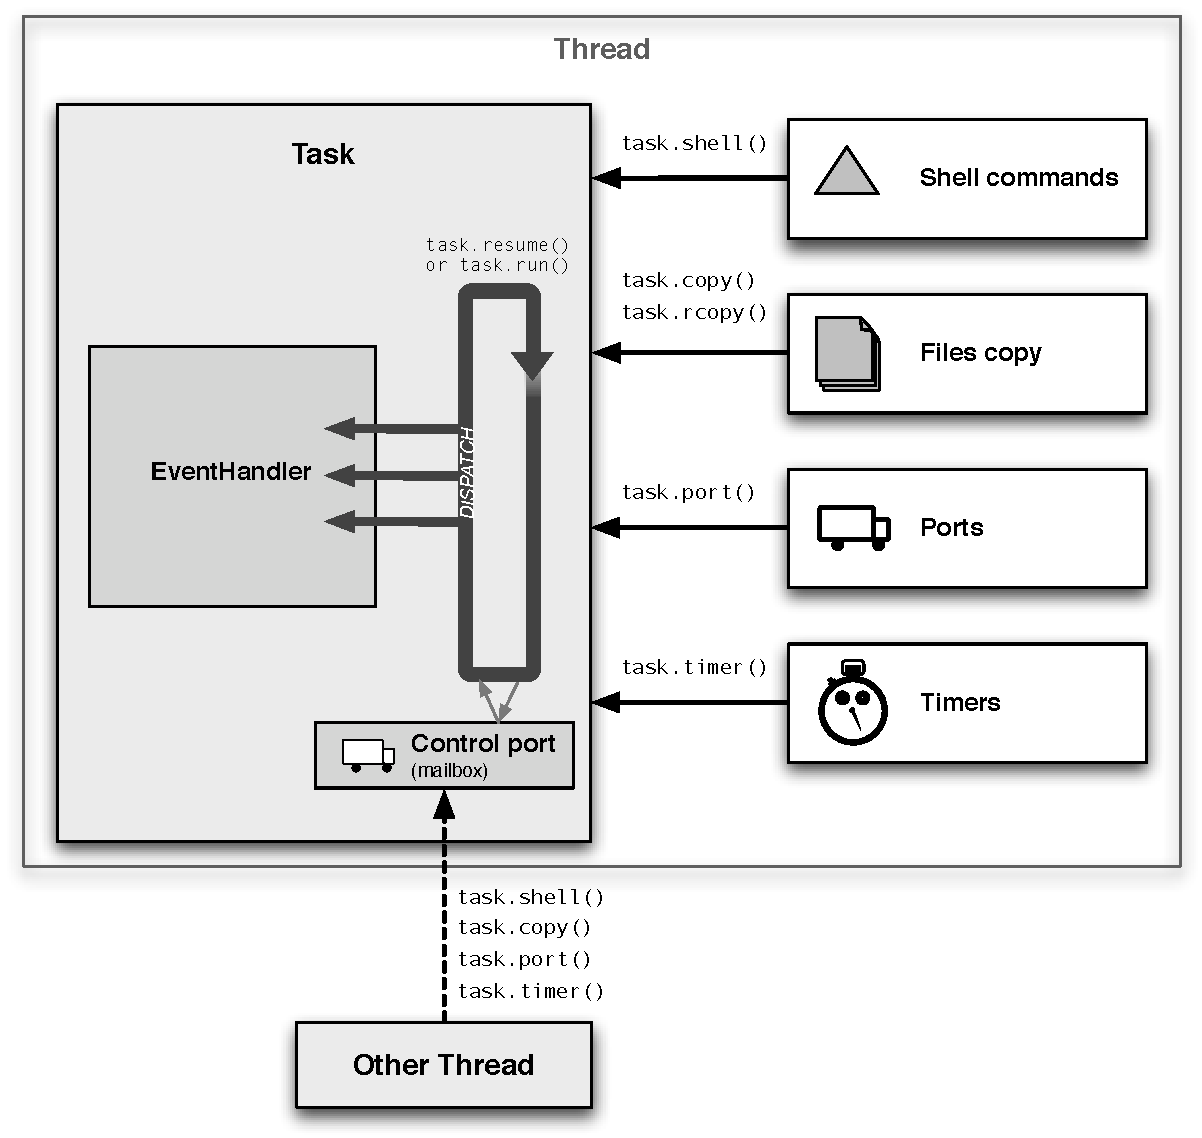
\includegraphics[scale=0.80]{TaskInterface}
\caption{Structure and interface overview of a ClusterShell \Task}
\label{TaskInterface}
\end{center}
\end{figure}

\begin{figure}[!ht]
\begin{center}
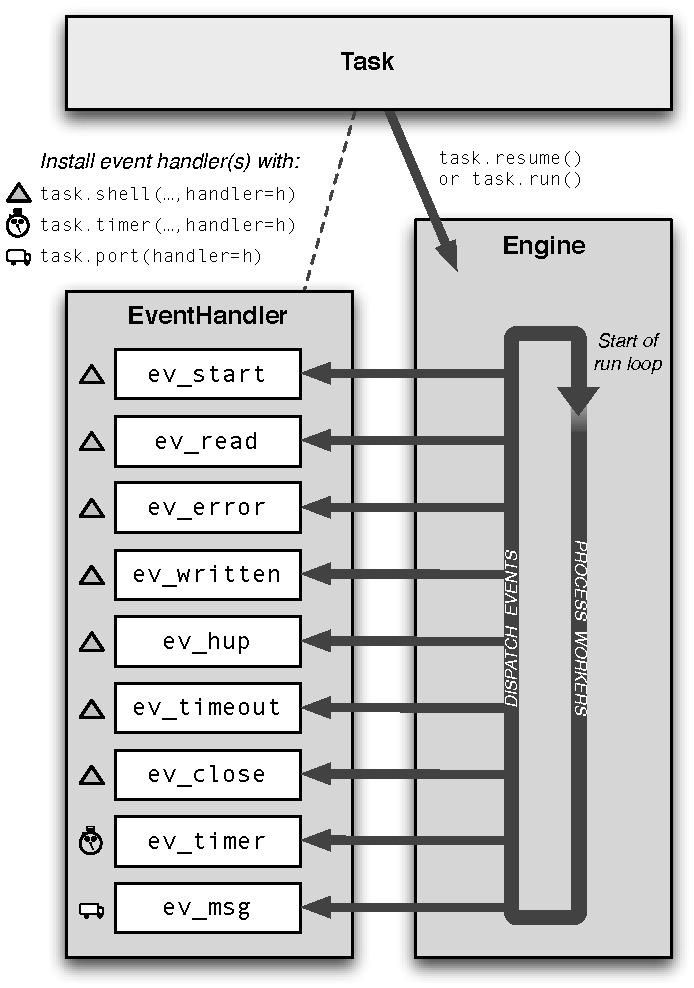
\includegraphics[scale=0.80]{TaskEvents}
\caption{Conceptual view of the thread execution flow of the \Task's underlying \Engine}
\label{TaskEvents}
\end{center}
\end{figure}


\subsection{Using \Task objects}

A \Task object provides the main interface for adding shell commands, files to copy or timer and then running it. Every thread has a single \Task object (and underlying \Engine object) associated with it. The \Task object is an instance of the ClusterShell.Task class.

\subsubsection{Getting a Task object}

To get the \Task object bound to the \textbf{current thread}, you use one of the following:
\begin{itemize}
\item Use the \lstinline+task_self()+ function available at the root of the Task module:

\begin{lstlisting}[breaklines=true, breakatwhitespace=true]
from ClusterShell.Task import task_self

task = task_self()
\end{lstlisting}
\item or use \lstinline+task = Task()+: Task objects are only instantiated when needed (new style Python class).
\end{itemize}
So for a single-threaded application, a Task is a simple singleton (which instance is also available through the \verb+task_self()+ function).

To get the Task object associated to a specific thread identified by the identifier tid, you use the following:
\begin{itemize}
\item \lstinline+task = Task(thread_id=tid)+
\end{itemize}
%If you plan to develop multi-threaded applications, please take a look at the the section \ref{threading} about threading safety.


\subsubsection{Configuring the \Task object}
\label{class-Task-configure}

Each \Task provides an info dictionary that shares both internal \Task-specific parameters and user-defined (key, value) parameters. Use the following \Task class methods to get or set parameters:
\begin{itemize}
\item \lstinline+def info(self, info_key, def_val=None)+
\item \lstinline+def set_info(self, info_key, value)+
\end{itemize}


For example, to configure the task debugging behavior with the \verb+set_info()+ method:
\begin{lstlisting}[breaklines=true, breakatwhitespace=true]
task.set_info('debug', True)
\end{lstlisting}

You can also use the \Task info dictionary to set your own \Task-specific key, value pairs. You may use any free keys but only keys starting with \lstinline+'USER_'+ are guaranteed not to be used by ClusterShell in the future.

\begin{figure}[!h]
\begin{center}
\begin{tabular}{|p{3.8cm}|p{2.9cm}|p{9.8cm}|} 
\hline 
\textbf{Info key string} & \textbf{Default value} & \textbf{Comment} \\
\hline
\lstinline+'debug'+ & \lstinline+False+ & Enable debugging support (boolean) \\
\hline
\lstinline+'print_debug'+ & (internal) & Default is to print debug lines to \emph{stdout} using \verb+print+. To override this behavior, set a function that takes two arguments (the task object and a string) as the value.\\
\hline
\lstinline+'fanout'+ & \lstinline+64+ & Ssh ``fanout'' window (integer) \\
\hline
\lstinline+'connect_timeout'+ & \lstinline+10+ & Value passed to ssh or pdsh (integer) \\
\hline
\lstinline+'command_timeout'+ & \lstinline+0+ (no timeout) & Value passed to ssh or pdsh (integer) \\
\hline
\end{tabular}
\end{center}
\caption{\Task info keys and their default values}
\end{figure}

\bigskip

Below is an example of \lstinline+'print_debug'+ override. As you can see, we set the function \lstinline+'print_csdebug(task, s)'+ as the value. When debugging is enabled, this function will be called for any debug text line. For example, this function searchs for any known patterns and print a modified debug line to \emph{stdout} when found.
\begin{figure}[!h]
\begin{center}
\begin{lstlisting}[breaklines=true, breakatwhitespace=true]
def print_csdebug(task, s):
   m = re.search("(\w+): SHINE:\d:(\w+):", s)
   if m:
       print "%s<pickle>" % m.group(0)
   else:
       print s

# Install the new debug printing function
task_self().set_info("print_debug", print_csdebug)
\end{lstlisting}
\end{center}
\end{figure}


\subsubsection{Submitting a shell command}
\label{taskshell}
You can submit a set of commands for local or distant execution in parallel with \lstinline+task.shell()+.

Local usage:
\begin{lstlisting}[breaklines=true, breakatwhitespace=true]
task.shell(command [, key=key] [, handler=handler] [, timeout=secs])
\end{lstlisting}
Distant usage:
\begin{lstlisting}[breaklines=true, breakatwhitespace=true]
task.shell(command, nodes=nodeset [, handler=handler] [, timeout=secs])
\end{lstlisting}

This method makes use of the default local or distant worker. ClusterShell uses a default Worker based on the Python Popen2 standard module to execute local commands, and a Worker based on \textit{ssh} (Secure SHell) for distant commands.

If the \Task is not running, the command is scheduled for later execution. If the \Task is currently running, the command is executed as soon as possible (depending on the current \emph{fanout}).

To set a per-worker timeout value (in seconds), just use the timeout parameter, for example:
\medskip
\begin{lstlisting}[breaklines=true, breakatwhitespace=true]
task.shell("uname -r", nodes=remote_nodes, handler=ehandler, timeout=5)
\end{lstlisting}

This is the prefered way to specify a command timeout. \lstinline+ev_timeout+ event is generated before the worker has finished to indicate that some nodes have timed out. You may then retrieve the nodes with \lstinline+worker.iter_keys_timeout()+.

\subsubsection{Submitting a file copy action}

Local file copy to distant nodes is supported. You can submit a copy action with \lstinline+task.copy()+.
\begin{lstlisting}[breaklines=true, breakatwhitespace=true]
task.copy(source, dest, nodes=nodeset [, handler=handler] 
	[, timeout=secs])
\end{lstlisting}

This method makes use of the default distant copy worker which is based on scp (Secure CoPy) which comes with OpenSSH.

If the \Task is not running, the copy is scheduled for later execution. If the \Task is currently running, the copy is started as soon as possible (depending on the current \emph{fanout}).

\subsubsection{Starting the \Task}

Before you run a \Task, you must add at least one worker (shell command, file copy) or timer to it. If a \Task does not have any worker to execute and monitor, it exits immediately when you try to run it with:

\begin{lstlisting}[breaklines=true, breakatwhitespace=true]
task.resume()
\end{lstlisting}

At this time, all previously submitted commands will start in the associated \Task's thread. From an library user point of view, the task's thread is blocked until the end of the command executions.

Please note that the special method \lstinline+Task.run()+ does a \lstinline+Task.shell()+ and a \lstinline+Task.resume()+ in once.

To set a \Task execution timeout, use the optional \lstinline+timeout+ parameter to set the timeout value in seconds. Once this time is elapsed when the Task is still running, , the running Task raises  a \lstinline+TimeoutError+ exception, cleaning by the way all scheduled workers and timers. Using such a timeout ensures that the Task will not exceed a given time for all its scheduled works. You can also configure per-worker timeout that generates an event (\lstinline+ev_timeout+) but will not raise an exception, allowing the Task to continue. Indeed, using a per-worker timeout is the prefered way for most applications.

\subsubsection{Exiting the Task}

If a Task does not have anymore scheduled worker or timer (for example, if you run one shell command and then it closes), it exits automatically from \lstinline+task.resume()+. Still, except from a signal handler, you can always call the following method to abort the Task execution:

\begin{lstlisting}[breaklines=true, breakatwhitespace=true]
task.abort()
\end{lstlisting}

For example, it is safe to call this method from an event handler within the task itself. On abort, all scheduled workers (shell command, file copy) and timers are cleaned and \lstinline+task.resume()+ returns, unblocking the Task's thread from a library user point of view. Please note that commands being executed remotely are not necessary stopped (this is due to \textit{ssh(1)} behavior).

\subsubsection{Configuring a timer}

A timer is bound to a Task (and its underlying Engine) and fires at a preset time in the future. Timers can fire either only once or repeatedly at fixed time intervals. Repeating timers can also have their next firing time manually adjusted (see API documentation).

A timer is not a real-time mechanism; it fires when the \Task's underlying \Engine to which the timer has been added is running and able to check if the timer's firing time has passed.

When a timer fires, the method \lstinline+ev_timer+ of the associated EventHandler is called.

To configure a timer, use the following (secs in seconds with floating point precision):
\medskip
\begin{lstlisting}[breaklines=true, breakatwhitespace=true]
task.timer(self, fire=secs, handler=handler [, interval=secs])
\end{lstlisting}

\subsubsection{Thread safety and Task objects}

ClusterShell is an event-based library and one of its advantage is to avoid the use of threads (and their safety issues), so it's mainly not thread-safe. When possible, avoid the use of threads with ClusterShell. However, it's sometimes not so easy, first because another library you want to use in some event handler is not event-based and may block the current thread (that's enough to break the deal). Also, in some cases, it could be useful for you to run several Tasks at the same time. Since version 1.1, ClusterShell provides support for launching a Task in another thread and some experimental support for multiple Tasks, but:
\begin{itemize}
\item you should ensure that a Task is configured and accessed from one thread at a time before it's running (there is no API lock/mutex protection),
\item once the Task is running, you should modify it only from the same thread that owns that Task (for example, you cannot call \lstinline+task.abort()+ from another thread).
\end{itemize}
The library provides two thread-safe methods and a function for basic Task interactions: \lstinline+Task.wait()+, \lstinline+task.join()+ and \lstinline+task_wait()+ (function defined at the root of the Task module). Please refer to the API documentation:
\begin{verbatim}
$ pydoc ClusterShell.Task
\end{verbatim}

\subsection{Configuring explicit Shell Worker objects}

We have seen in section \ref{taskshell} how to easily submit shell commands to the Task. The \lstinline+task.shell()+ command returns an already scheduled Worker object. It is possible to instantiate the Worker object explicitly, for example:
\medskip
\begin{lstlisting}[breaklines=true, breakatwhitespace=true]
from ClusterShell.Worker.Ssh import WorkerSsh

worker = WorkerSsh('node3', command="/bin/echo alright")
\end{lstlisting}

To be used in a Task, add the worker to it with:
\medskip
\begin{lstlisting}[breaklines=true, breakatwhitespace=true]
task.schedule(worker)
\end{lstlisting}

\pagebreak[2]

If you have pdsh installed, you can use it by easily switching to the Pdsh worker, which should behave the same manner as the Ssh worker:
\medskip
\begin{lstlisting}[breaklines=true, breakatwhitespace=true]
from ClusterShell.Worker.Pdsh import WorkerPdsh

worker = WorkerPdsh('node3', command="/bin/echo alright")
\end{lstlisting}


\newpage

\section{Programming examples}

\subsection{Remote command example (sequential mode)}

The following example shows how to send a command on some nodes, how to get a specific buffer and how to get gathered buffers.
\medskip
\begin{lstlisting}[breaklines=true, breakatwhitespace=true]
from ClusterShell.Task import task_self
task = task_self()

task.shell("/bin/uname -r", nodes="green[36-39,133]")

task.resume()

print worker.node_buffer("green37")

for buf, nodes in task.iter_buffers():
	print nodes, buf

\end{lstlisting}

Result:
\begin{verbatim}
2.6.25.11
['green37', 'green38', 'green36', 'green39'] 2.6.25.11
['green133'] 2.6.25
\end{verbatim}

\subsection{Remote command example with live output (event-based mode)}

The following example shows how to use the event-based programmation model by installing an EventHandler and listening for \lstinline+ev_read+ events. The goal here is to print standard outputs of ``uname -a'' commands during their execution.
\medskip
\begin{lstlisting}[breaklines=true, breakatwhitespace=true]
from ClusterShell.Task import task_self
from ClusterShell.Event import EventHandler

class MyHandler(EventHandler):
   def ev_read(self, worker):
       node, buf = worker.last_read()
       print "%s: %s" % (node, buf)

task = task_self()

# Submit command, install event handler for this command and run task
task.run("/bin/uname -a", nodes="fortoy[32-159]", handler=MyHandler())
\end{lstlisting}


\subsection{\texttt{check\_nodes.py} example script}

The following script is available as an example in the source repository and is usually packaged with ClusterShell.
\medskip
\begin{lstlisting}[breaklines=true, breakatwhitespace=true]
#!/usr/bin/python
# check_nodes.py: ClusterShell simple example script.
#
# This script runs a simple command on remote nodes and report node
# availability (basic health check) and also min/max boot dates.
# It shows an example of use of Task, NodeSet and EventHandler objects.
# Feel free to copy and modify it to fit your needs.
#
# Usage example: ./check_nodes.py -n node[1-99]

import optparse
from datetime import date, datetime
import time

from ClusterShell.Event import EventHandler
from ClusterShell.NodeSet import NodeSet
from ClusterShell.Task import task_self


class CheckNodesResult:
    """Our result class"""
    def __init__(self):
        """Initialize result class"""
        self.nodes_ok = NodeSet()
        self.nodes_ko = NodeSet()
        self.min_boot_date = None
        self.max_boot_date = None

    def show(self):
        """Display results"""
        if self.nodes_ok:
            print "%s: OK (boot date: min %s, max %s)" % \
                (self.nodes_ok, self.min_boot_date, self.max_boot_date)
        if self.nodes_ko:
            print "%s: FAILED" % self.nodes_ko

class CheckNodesHandler(EventHandler):
    """Our ClusterShell EventHandler"""
    
    def __init__(self, result):
        """Initialize our event handler with a ref to our result object."""
        EventHandler.__init__(self)
        self.result = result

    def ev_read(self, worker):
        """Read event from remote nodes"""
        node = worker.current_node
        # this is an example to demonstrate remote result parsing
        bootime = " ".join(worker.current_msg.strip().split()[2:])
        date_boot = None
        for fmt in ("%Y-%m-%d %H:%M",): # formats with year
            try:
                # datetime.strptime() is Python2.5+, use old method instead
                date_boot = datetime(*(time.strptime(bootime, fmt)[0:6]))
            except ValueError:
                pass
        for fmt in ("%b %d %H:%M",):    # formats without year
            try:
                date_boot = datetime(date.today().year, \
                    *(time.strptime(bootime, fmt)[1:6]))
            except ValueError:
                pass
        if date_boot:
            if not self.result.min_boot_date or \
                self.result.min_boot_date > date_boot:
                self.result.min_boot_date = date_boot
            if not self.result.max_boot_date or \
                self.result.max_boot_date < date_boot:
                self.result.max_boot_date = date_boot
            self.result.nodes_ok.add(node)
        else:
            self.result.nodes_ko.add(node)

    def ev_timeout(self, worker):
        """Timeout occurred on some nodes"""
        self.result.nodes_ko.add( \
        	NodeSet.fromlist(worker.iter_keys_timeout()))

    def ev_close(self, worker):
        """Worker has finished (command done on all nodes)"""
        self.result.show()


def main():
    """ Main script function """
    # Initialize option parser
    parser = optparse.OptionParser()
    parser.add_option("-d", "--debug", action="store_true", dest="debug",
        default=False, help="Enable debug mode")
    parser.add_option("-n", "--nodes", action="store", dest="nodes",
        default="@all", help="Target nodes (default @all group)")
    parser.add_option("-f", "--fanout", action="store", dest="fanout",
        default="128", help="Fanout window size (default 128)", type=int)
    parser.add_option("-t", "--timeout", action="store", dest="timeout",
        default="5", help="Timeout in seconds (default 5)", type=float)
    options, _ = parser.parse_args()

    # Get current task (associated to main thread)
    task = task_self()
    nodes_target = NodeSet(options.nodes)
    task.set_info("fanout", options.fanout)
    if options.debug:
        print "nodeset : %s" % nodes_target
        task.set_info("debug", True)

    # Create ClusterShell event handler
    handler = CheckNodesHandler(CheckNodesResult())

    # Schedule remote command and run task (blocking call)
    task.run("who -b", nodes=nodes_target, handler=handler, \
        timeout=options.timeout)


if __name__ == '__main__':
    main()
\end{lstlisting}


\newpage

\nocite{*}

\bibliographystyle{frplain}

\bibliography{abrev,biblio}

\end{document}
